\documentclass[11pt]{article}
\usepackage{geometry}
\usepackage{graphicx}
\usepackage{wrapfig}
\usepackage{float}
\usepackage{caption}
\usepackage{subcaption}
\usepackage[T1]{fontenc}
\usepackage[utf8]{inputenc}
\usepackage{helvet}
\renewcommand{\familydefault}{\sfdefault}
%\usepackage{titlesec}
%\titlespacing\section{1pt}{12pt plus 2pt minus 2pt}{1pt plus 2pt minus 2pt}
%\titlespacing\subsection{1pt}{12pt plus 2pt minus 2pt}{pt plus 2pt minus 2pt}
%\titlespacing\subsubsection{5pt}{12pt plus 2pt minus 2pt}{1pt plus 2pt minus 2pt}
%\usepackage{float}
\usepackage{booktabs}
\usepackage[hidelinks]{hyperref}
\usepackage{hyperref}
\usepackage{float}
\hypersetup{
	colorlinks=true,
	linkcolor=blue,
	filecolor=magenta,      
	urlcolor=cyan,
	pdftitle={Overleaf Example},
	pdfpagemode=FullScreen,
}
\setcounter{tocdepth}{4}
\urlstyle{same}
\geometry{margin=0.5in}
%opening
%\titleformat*{\section}{\small\bfseries}
\bibliographystyle{unsrt}
\author{Ethan Holleman}
\title{Variable region design and cloning}

\begin{document}

\maketitle
\begin{abstract}
	Abstract text here
\end{abstract}

\tableofcontents
\pagebreak

\section{Background}

R-loops are prevalent, functional important, non-B DNA structures that form co-transcriptionally when the nascent RNA strand hybridizes back to the DNA template forming a DNA-RNA hybrid \cite{chedin_nascent_2016}. 

\begin{figure}[H]
	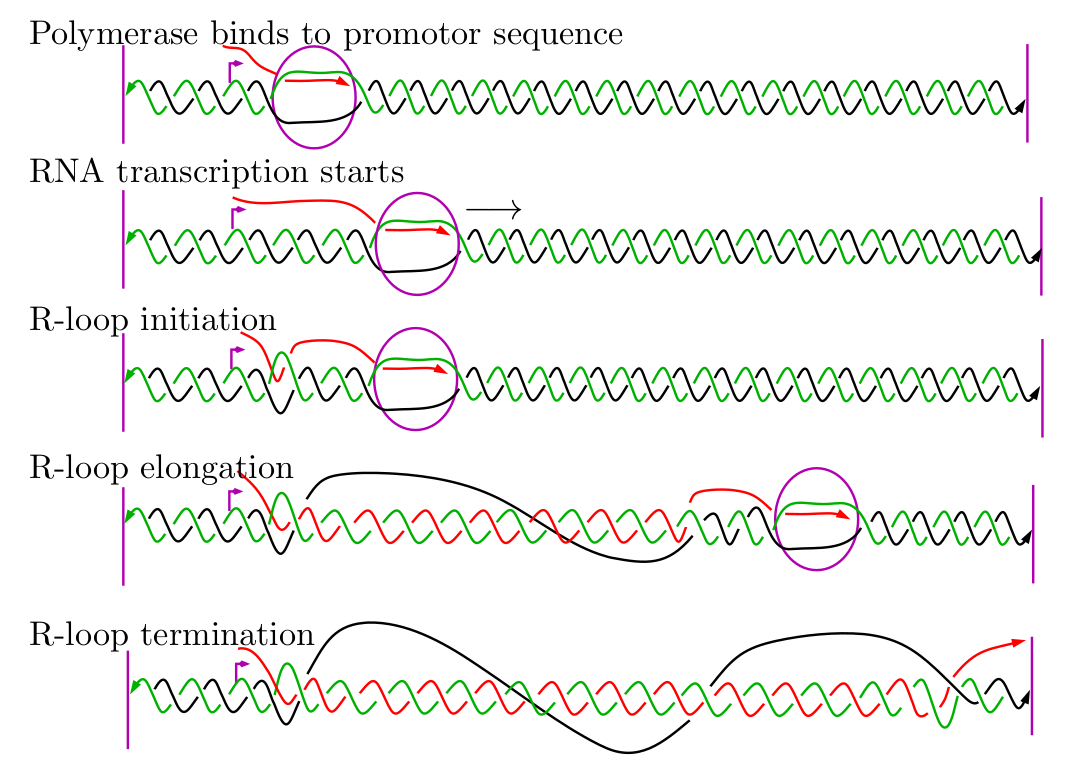
\includegraphics[width=12cm]{images/r-loops/rloop_stages.png}
	\centering
	\caption{Stages of R-loop formation. The encircled region represents the transcription bubble. The polymerase moves from left to right, starting at the promoter region (purple arrow). The upper strand (in red) in the bubble corresponds to the nascent RNA transcript, generated in the 5' to 3' direction. The R-loop initiates in frame 3, elongates in frame 4, and terminates in frame 5. Vazquez, Chedin and Natasa, 2020.}
	\label{fig:1}
\end{figure}




\section{Insert design}

The overall goal of this series of experiments is to transcribe carefully controlled DNA sequences, referred to as inserts, in order to systematically observe the effects of these sequences on R-loop formation \emph{in vitro}. Inserts are composed of two types of DNA components, the variable region and flanking infrastructure regions. The variable region contains the sequence we are interested in observing R-loop dynamics over. Infrastructure sequences are additional nucleotide blocks that allow for the insertion of variable regions into specific plasmid backbones in a modular fashion. 

\begin{figure}[H]
	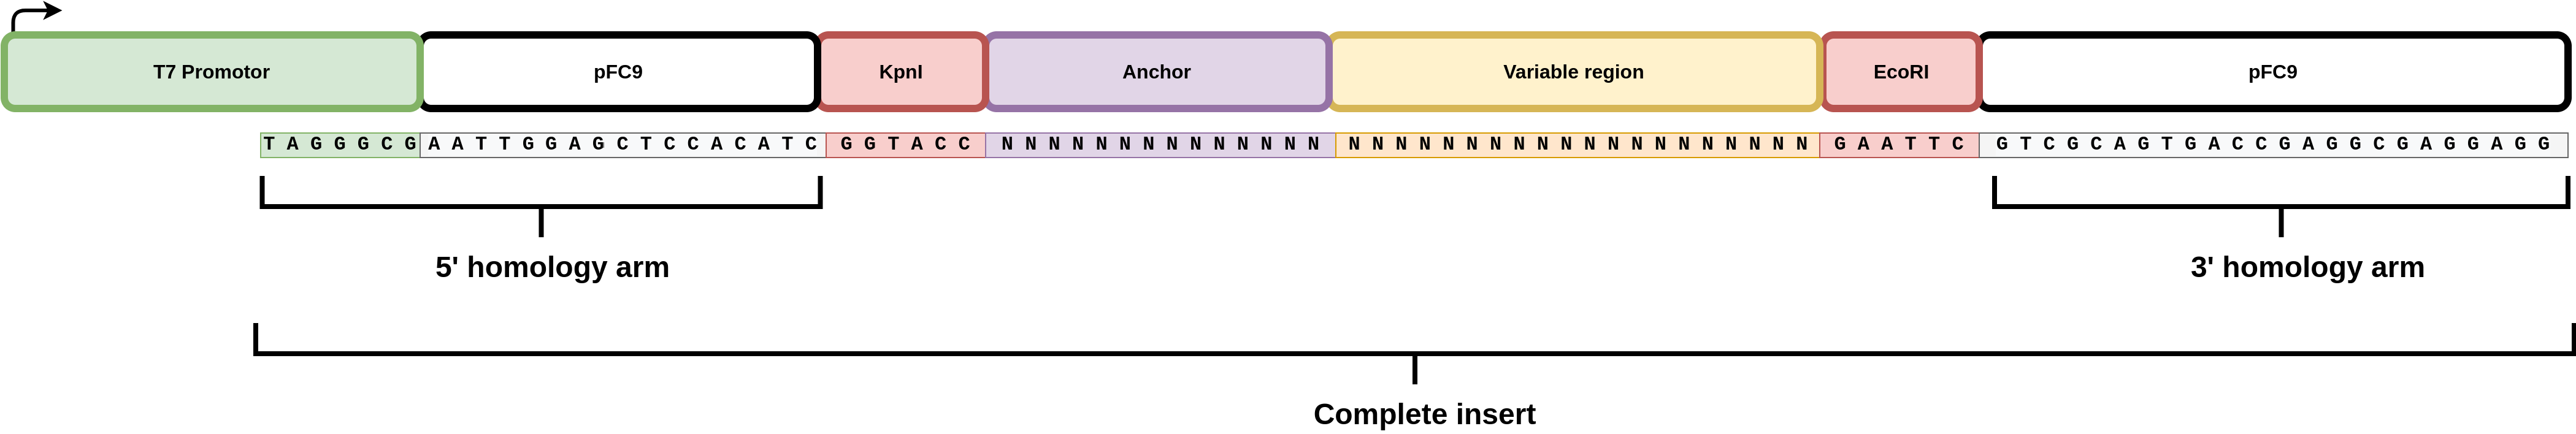
\includegraphics[width=16cm]{images/variable_region/construct_diagrams-Detailed-Insert.png}
	\centering
	\caption{Diagram of a complete insert. Colored boxes represent features insert sequences are derived from while colored sequences represent the actual nucleotide sequence.}
	\label{fig:1}
\end{figure}

From right to left (5' to 3') each insert will contain a 5' homology arm with complementary to the last 7 nucleotides of the T7 promoter, 17 nucleotides complementary to the pFC9 plasmid immediately downstream of the T7 promoter for a total of 24 bp. This will be followed by a KpnI recognition site, and an "anchor" region will will be composed of a constant sequence which can be utilized for targeting by PCR primers. The following region will contain the variable region which defines the identity of each complete insert. Finally a EcoRI recognition site and 24 taken from the region downstream of pFC9's EcoRI recognition site will be included. This design will allow for insertion of variable regions in either forward or reverse orientations using combinations of Gibson and restriction enzyme cloning, as well as allowing for later extraction via PCR or restriction enzymes. Specific methodolgies are discussed in greater detail in section \ref{}. Each insert will be completely synthesized as double strand DNA from an outside company and therefore require no additional assembly. 

\subsection{Insert components}

\subsubsection{5' homology arm and KpnI recognition site}

The first 30 bp of each insert will be composed of the 5' homology arm and a KpnI recognition site. These sequences are included to facilitate Gibson and restriction enzyme cloning into pFC9 and pFC9 respectively. These 30 bp are taken directly from nucleotides 27 - 56 of pFC9.

\begin{figure}[h]
	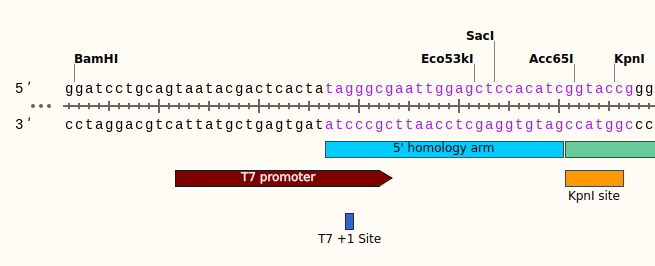
\includegraphics[width=12cm]{images/variable_region/5_homology_arm.png}
	\centering
	\caption{Location in pFC9 from which the 5' homology arm and KpnI site are modeled after. The entire 30 bp sequence is shown in purple with the 5' homology arm highlighted as a feature in blue and the KnpI site in orange.}
	\label{fig:1}
\end{figure}

This strategy will mean recognition sites for Eco53KI, SacI and Acc65I will be included in the 5' homology arms but none of these enzymes will be utilized in any cloning protocols and so only the KpnI site is noted in diagrams.


\subsubsection{Anchor}

The anchor region serves as a constant sequence that will always be present in any final assembled construct adjacent to the 5' end of the variable region. Having this region within the insertion sequence means for a given plasmid backbone, at most 1 pair of primers will be required to amplify any sequence downstream of the 3' end of the anchor. This is useful when working with libraries containing all insertion sequences as each unique insertion will not require its own primer pair to amplify. This utility is more explicitly shown in sections \ref{sec:tac-init} and \ref{sec:tac-termination}. 

Since this region is intended to be used as part of a PCR primer it is selected from candidate random sequences that satisfy the requirements below.

\begin{itemize}
	\item Does not contain any common sub-strings of minimun length equal to 75\% of the anchor's own length with any variable region or plasmid backbone.
	\item Does not contain the recognition sites for any restriction enzyme used in any relevant cloning procedure (see table \ref{tab:enzymes}).
	\item Has a melting temperature estimated by using \href{https://biopython.org/docs/1.75/api/Bio.SeqUtils.MeltingTemp.html#Bio.SeqUtils.MeltingTemp.Tm_GC}{nearest neighbor thermodynamics} of at least 50\textdegree C.
\end{itemize}

\subsubsection{Variable regions}

Each insert will contain 1 variable region which will be designed to test the effects of different sequence properties on R-loop dynamics, namely GC / AT skew, GC content and G / C clustering. Each variable region will be 200 bp in length. Twenty nine different variable regions with the properties described in table \ref{table:1} will be generated using the \href{https://github.com/EthanHolleman/plasmid-VR-design}{variable region design workflow}. Each variable region, as part of the larger insertion sequence, will be cloned downstream of a promoter so it is transcribed in the forward direction. 

\begin{table}
\centering
\caption{Properties of all syntheized inserts. The G clustering number refers to the number of G nucleotides in a given cluster with 0 being no clustering.}
\label{table:1}
\begin{tabular}{rrrrrr}
\toprule=
 GC Skew &  AT Skew &  GC Content &  G Clustering &  Reverse Complement &  Insert Number \\
\midrule
     0.2 &      0.0 &         0.4 &             0 &                   1 &              0 \\
     0.1 &      0.0 &         0.3 &             0 &                   0 &              1 \\
     0.6 &      0.0 &         0.6 &             0 &                   0 &              2 \\
     0.4 &      0.0 &         0.3 &             0 &                   1 &              3 \\
     0.2 &      0.0 &         0.3 &             0 &                   1 &              4 \\
     0.0 &      0.0 &         0.3 &             0 &                   1 &              5 \\
     0.0 &      0.0 &         0.6 &             0 &                   0 &              6 \\
     0.6 &      0.0 &         0.5 &             0 &                   0 &              7 \\
     0.1 &      0.0 &         0.6 &             0 &                   0 &              8 \\
     0.4 &      0.0 &         0.6 &             0 &                   0 &              9 \\
     0.2 &      0.0 &         0.6 &             0 &                   0 &             10 \\
     0.0 &      0.0 &         0.5 &             0 &                   1 &             11 \\
     0.6 &      0.0 &         0.4 &             0 &                   0 &             12 \\
     0.0 &      0.0 &         0.4 &             0 &                   1 &             13 \\
     0.1 &      0.0 &         0.5 &             0 &                   0 &             14 \\
     0.6 &      0.0 &         0.3 &             0 &                   0 &             15 \\
     0.4 &      0.0 &         0.5 &             0 &                   1 &             16 \\
     0.2 &      0.0 &         0.5 &             0 &                   1 &             17 \\
     0.1 &      0.0 &         0.4 &             0 &                   0 &             18 \\
     0.4 &      0.0 &         0.4 &             0 &                   1 &             19 \\
     0.4 &      0.0 &         0.6 &             2 &                   1 &             20 \\
     0.4 &      0.2 &         0.6 &             2 &                   1 &             21 \\
     0.4 &      0.4 &         0.6 &             2 &                   1 &             22 \\
     0.4 &      0.0 &         0.6 &             3 &                   1 &             23 \\
     0.4 &      0.2 &         0.6 &             3 &                   1 &             24 \\
     0.4 &      0.4 &         0.6 &             3 &                   1 &             25 \\
     0.4 &      0.0 &         0.6 &             4 &                   1 &             26 \\
     0.4 &      0.2 &         0.6 &             4 &                   1 &             27 \\
     0.4 &      0.4 &         0.6 &             4 &                   1 &             28 \\
\bottomrule
\end{tabular}
\end{table}


A subset of the variable regions will also be cloned further downstream of the same promoter species and oriented so the reverse complement of the sequence is transcribed in order to access these regions capacity for R-loop termination. The properties of the transcripts of these sequences are listed in table \ref{table:2}. 

\begin{table}[H]
\centering
\caption{}
\label{table:2}
\begin{tabular}{rrrrr}
\toprule
 GC Skew &  AT Skew &  GC Content &  C Clustering &  Reverse Complement of Insert \\
\midrule
    -0.2 &     -0.0 &         0.4 &             0 &                             0 \\
    -0.4 &     -0.0 &         0.3 &             0 &                             3 \\
    -0.2 &     -0.0 &         0.3 &             0 &                             4 \\
    -0.0 &     -0.0 &         0.3 &             0 &                             5 \\
    -0.0 &     -0.0 &         0.5 &             0 &                            11 \\
    -0.0 &     -0.0 &         0.4 &             0 &                            13 \\
    -0.4 &     -0.0 &         0.5 &             0 &                            16 \\
    -0.2 &     -0.0 &         0.5 &             0 &                            17 \\
    -0.4 &     -0.0 &         0.4 &             0 &                            19 \\
    -0.4 &     -0.0 &         0.6 &             2 &                            20 \\
    -0.4 &     -0.2 &         0.6 &             2 &                            21 \\
    -0.4 &     -0.4 &         0.6 &             2 &                            22 \\
    -0.4 &     -0.0 &         0.6 &             3 &                            23 \\
    -0.4 &     -0.2 &         0.6 &             3 &                            24 \\
    -0.4 &     -0.4 &         0.6 &             3 &                            25 \\
    -0.4 &     -0.0 &         0.6 &             4 &                            26 \\
    -0.4 &     -0.2 &         0.6 &             4 &                            27 \\
    -0.4 &     -0.4 &         0.6 &             4 &                            28 \\
\bottomrule
\end{tabular}
\end{table}


The cloning experiments required to produce these termination constructs will be undertaken after initiation experiments are completed. This will allow for the identification of a strong initiation sequence that can be used to reliability initiated R-loops in order to study their downstream termination. 

\begin{table}
\centering
\caption{}
\label{table:3}
\begin{tabular}{rr}
\toprule
 Total synthesized inserts &  Total contructs \\
\midrule
                        29 &               47 \\
\bottomrule
\end{tabular}
\end{table}


While the global sequence properties for each variable region are well defined, properties such as GC-skew, content or clustering do not determine what nucleotide should occur at position \emph{n} in a given sequence. In this way, the parameters that define and separate each variable region can be thought of as bounding the set of all possible nucleotide sequences of length 200. In order one specific sequence from this set we can sample a large number of sequences and access each one with metrics relevant to the realities of the cloning protocols and R-loop formation. 

\begin{figure}[H]
	\includegraphics[width=18cm]{images/plots/VR-1.all_ranked.png}
	\centering
	\caption{}
	\label{ranking}
\end{figure}


\paragraph{Restriction enzyme recognition sites}

Over the course of all planned cloning experiments, all the restriction enzymes in table \ref{} will be utilized in some capacity. It is therefore critical that the inserts are not cut unexpectedly within the variable region by any of these enzymes. Accordingly, before passing on for further downstream analysis potential variable regions containing any of these recognition sites were thrown out. 

\begin{table}[H]
	\caption{}
	\label{tab:enzymes}
	\centering
	\begin{tabular}{@{}ll@{}}
		\toprule
		Enzyme  & Recognition sequence \\ \midrule
		KnpI    & GGTACC               \\
		EcoRI   & GAATTC               \\
		HindIII & AAGCTT               \\ \bottomrule
	\end{tabular}
\end{table}


\paragraph{Predicted R-loop probability}

Previous Chedin lab member Dr. Robert Stolz developed rlooper, a physics based equilibrium model for predicting the probability of R-loop formation over a given DNA sequence. Rlooper output includes a predicted probability of R-loop formation at each base in the input sequence, and the calculated average free energy from all R-loops overlapping that particular nucleotide. Since, for this analysis, we prefer to select variable regions that are more likely to form R-loops these metrics are also used to compare and rank candidate variable regions with highest ranking sequences having low mean local average energy and high average R-loop probability compared to all sequences generated with the same parameters. 

\begin{figure}[H]
	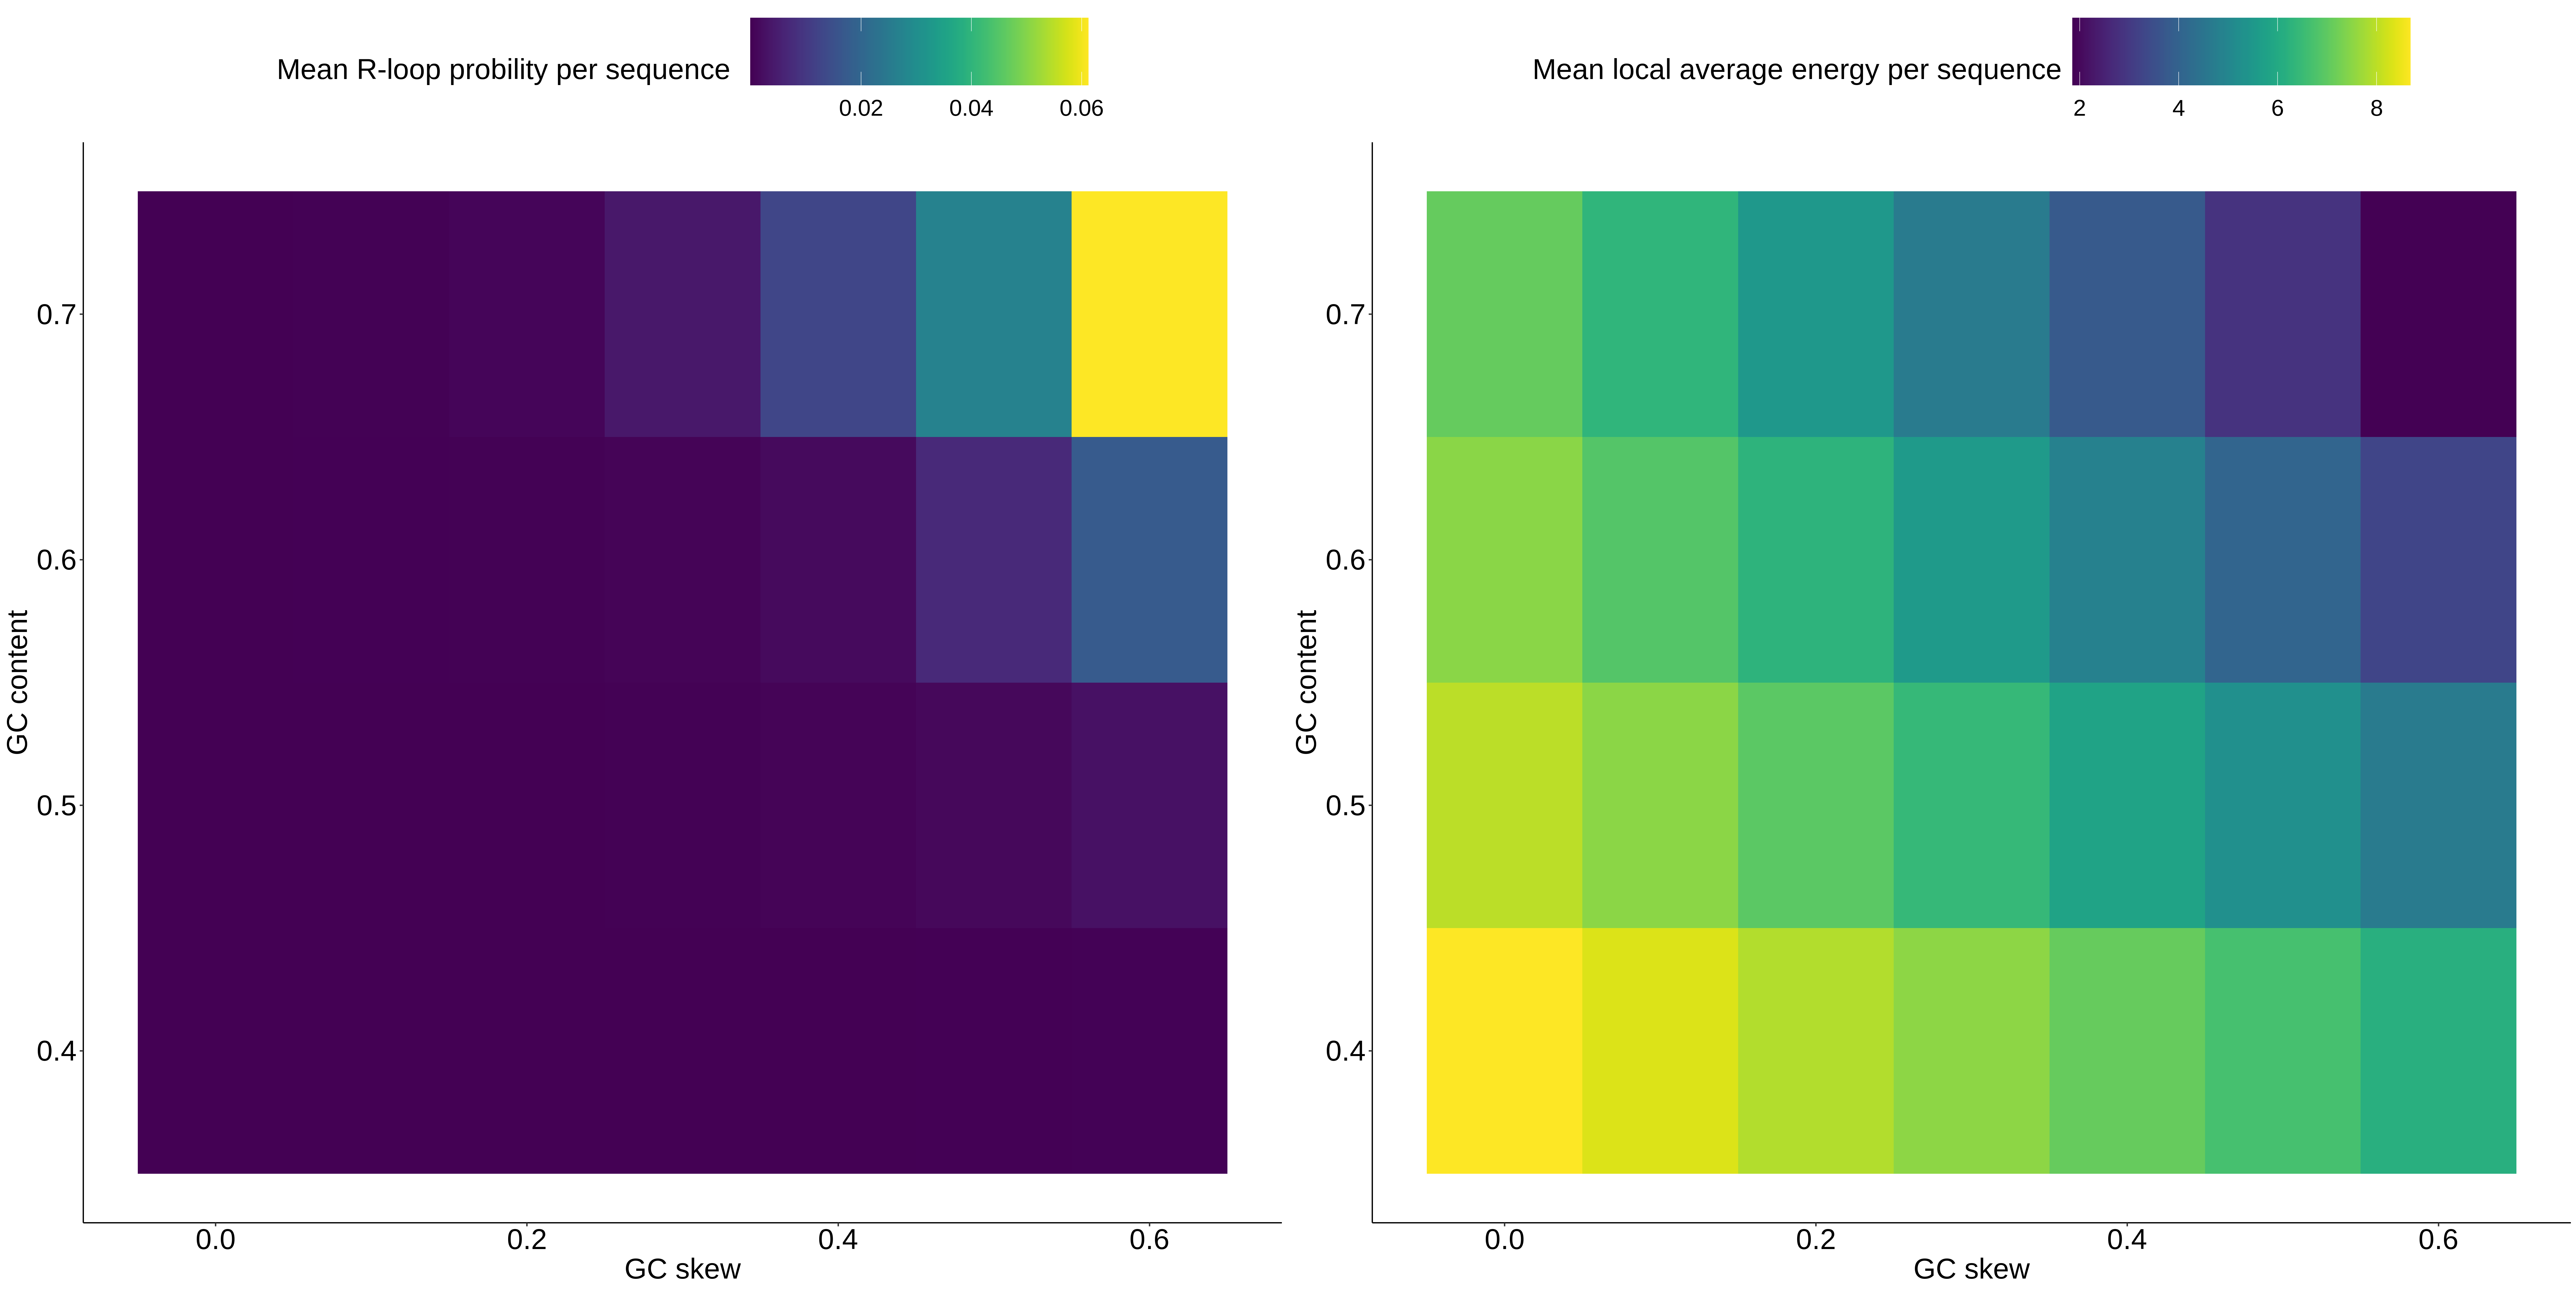
\includegraphics[width=14cm]{images/plots/rlooper_expect_tile.png}
	\centering
	\caption{Heatmaps showing mean R-loop probability (left) and mean local average energy per sequence (right) for 100 sequences of length 200 at various levels of both GC skew and content. As GC skew and GC content increase, the mean R-loop probability also increase while the mean local average energy tends to decrease which aligns with the basic expectation that increased GC skew and content favor R-loop formation.}
	\label{fig:rlooper-expect}
\end{figure}

Both local average energy and somewhat consequentially, mean R-loop probability are sensitive to both the GC skew and content of the input sequence (fig \ref{fig:rlooper-expect}). Comparing between sequences generated with the same parameters and therefore GC skew and content ensures that we are mainly evaluating how the arrangement of a particular set of nucleotides is predicted in generally effect the likelihood of R-loop formation.



\paragraph{RNA secondary structure}

Significant amounts of RNA secondary structure, especially large hairpins, can be expected to reduce the likelihood of R-loop formation by causing competition for binding to the nascent RNA strand between itself and the DNA template. 


\begin{figure}[H]
	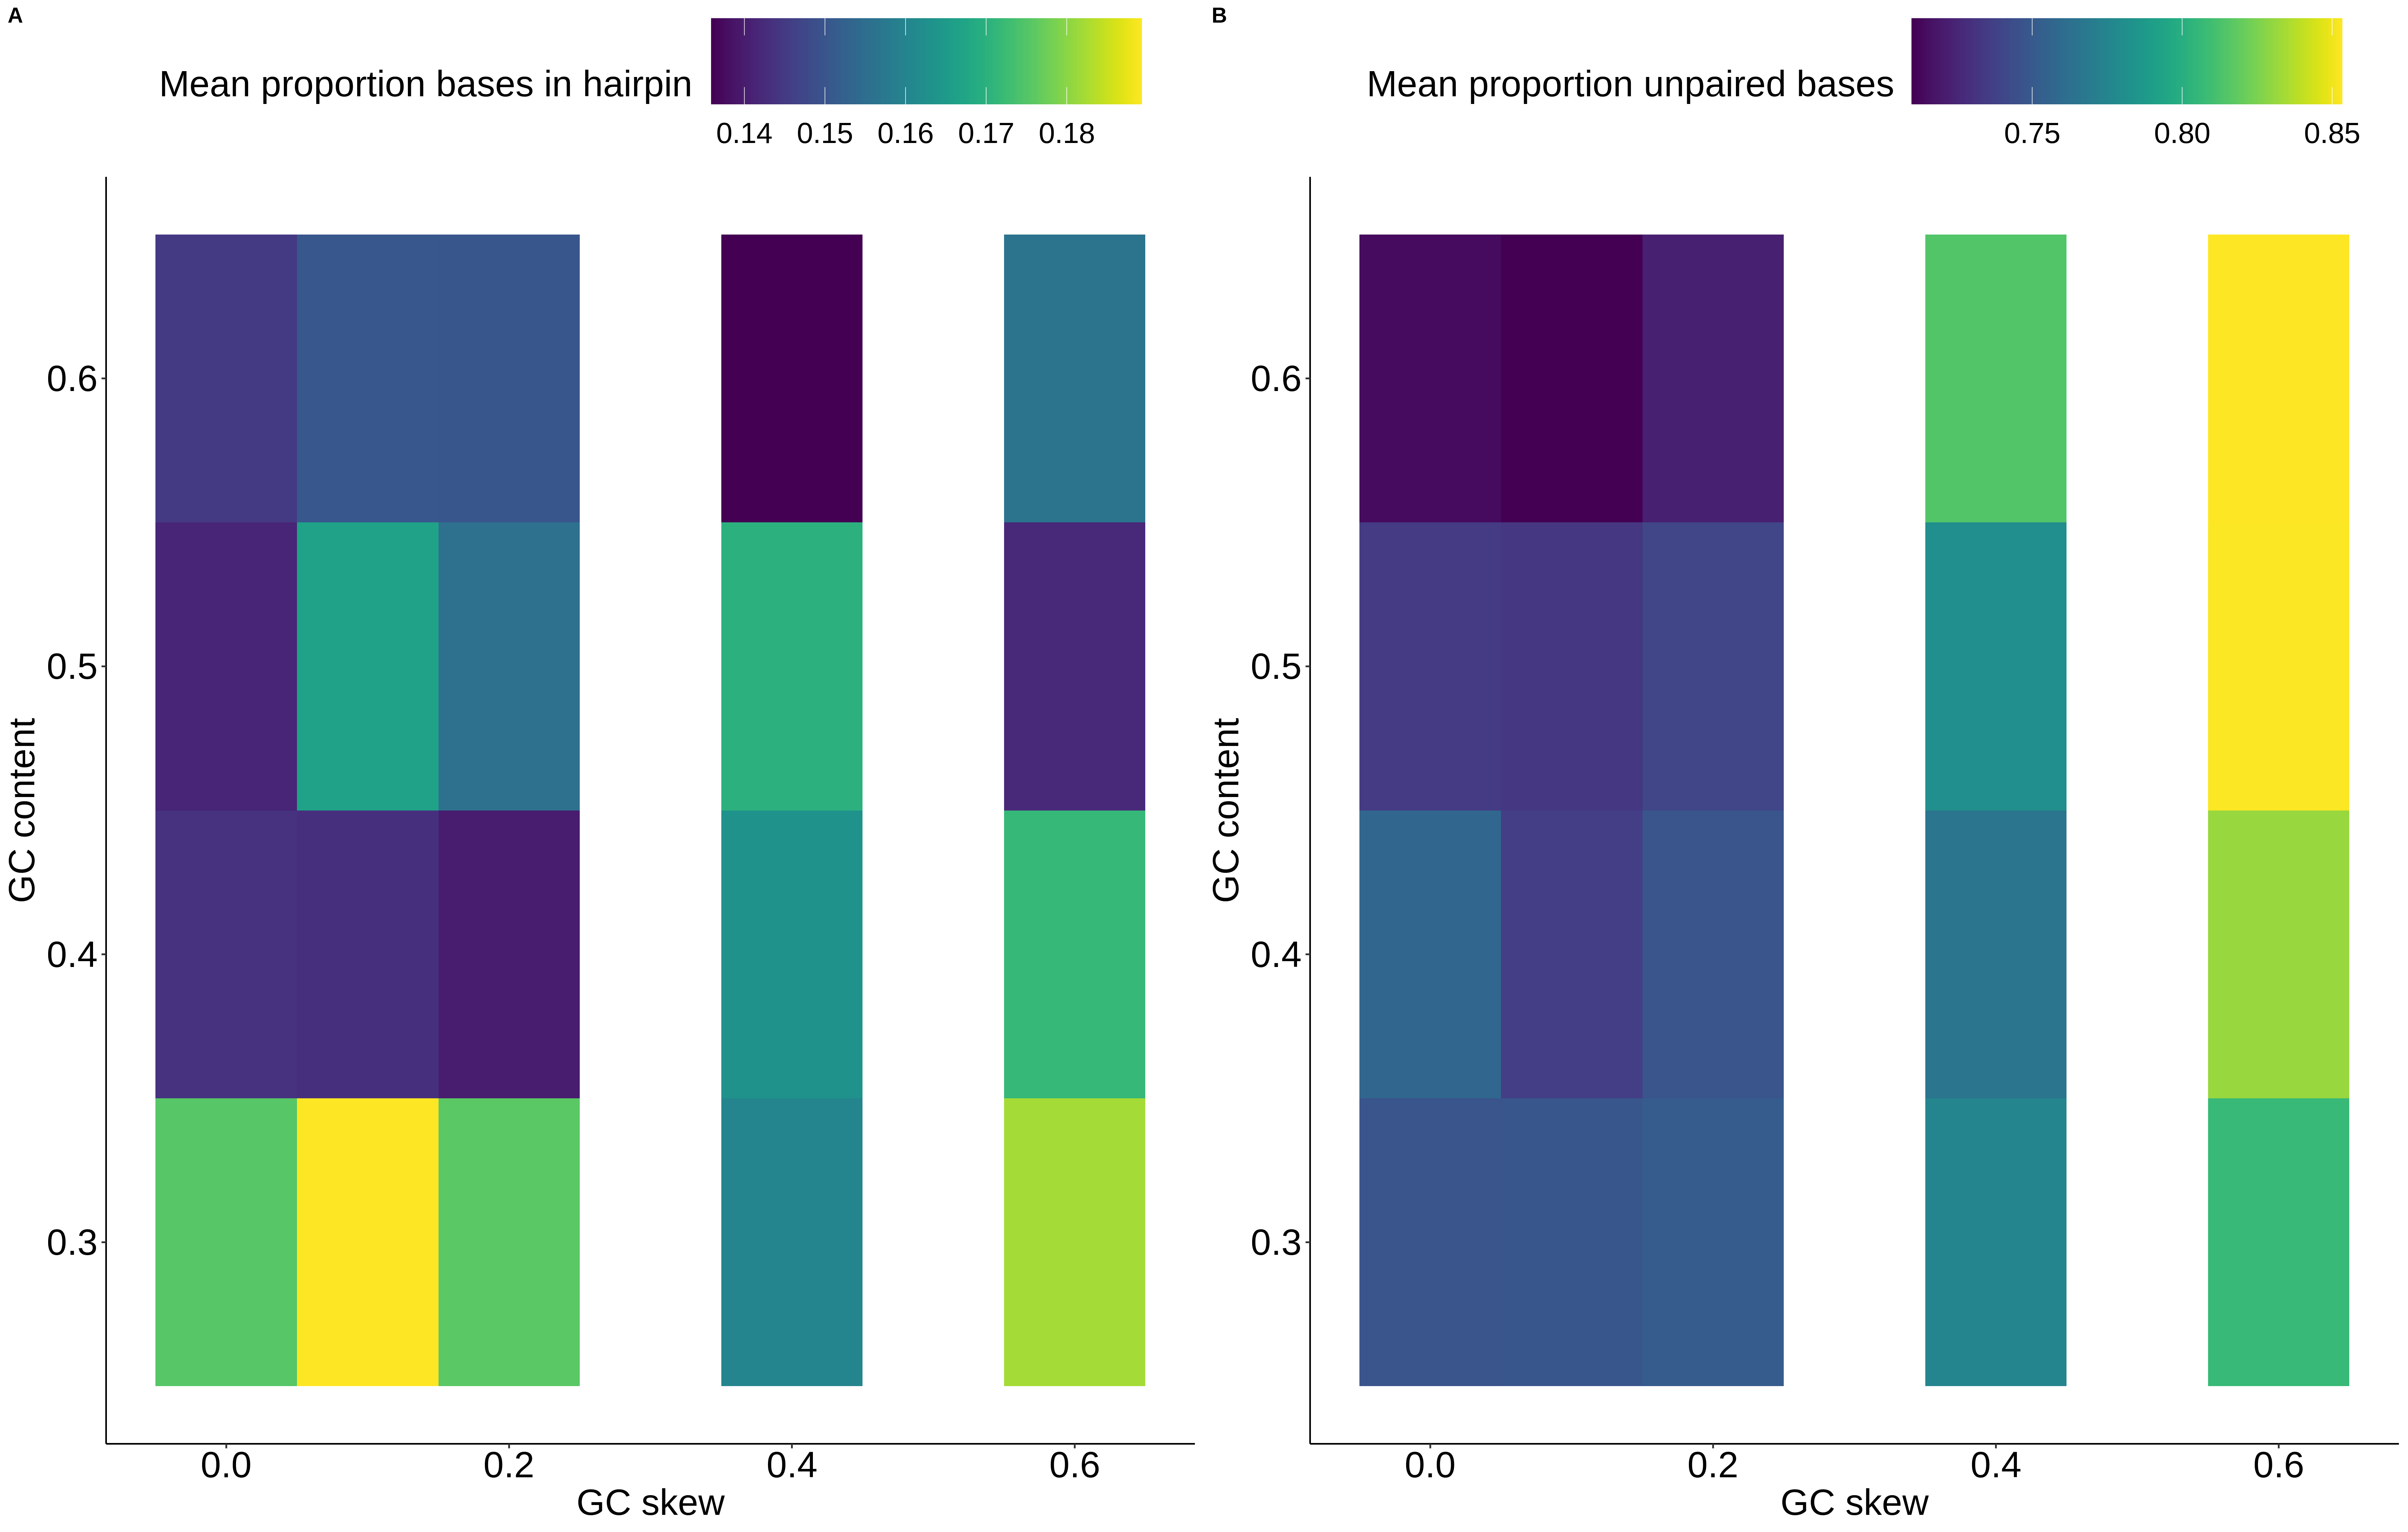
\includegraphics[width=10cm]{images/plots/rna_secondary_structure_temp.png}
	\centering
	\caption{Sequence of the 3' homology arm and EcoRI site. The complete sequence is highlighted in purple.}
	\label{fig:3_prime_arm}
\end{figure}

Need to update the above with same datapoints as R-looper

\subsubsection{EcoRI site and 3' homology arm}

The final 20 nucleotides of each insert will be composed of a EcoRI recognition site (6 bp) and the 3' homology arm (24 bp). 

\begin{figure}[H]
	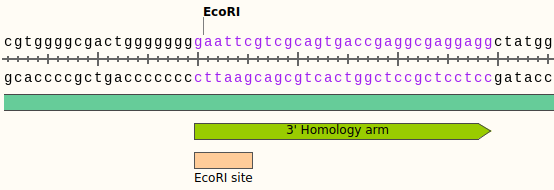
\includegraphics[width=10cm]{images/variable_region/3_homology_arm.png}
	\centering
	\caption{Sequence of the 3' homology arm and EcoRI site. The complete sequence is highlighted in purple.}
	\label{fig:3_prime_arm}
\end{figure}



\section{Assembly of DNA inserts}

Complete insert sequences will be cloned into three different plasmid backbones: pFC9 (fig \ref{fig:map_pFC8}), pFC8 (fig \ref{fig:map_pFC8}), and pFC53tacT$_1$T$_2$ (fig \ref{fig:map_pFC53tacT1T2}). pFC9 will be utilized for testing R-loop initiation, pFC8 for R-loop termination and pFC53tacT$_1$T$_2$ for multiple round and single-round transcription versions of both initiation and termination experiments with Tac polymerase. 


\begin{figure}[H]
	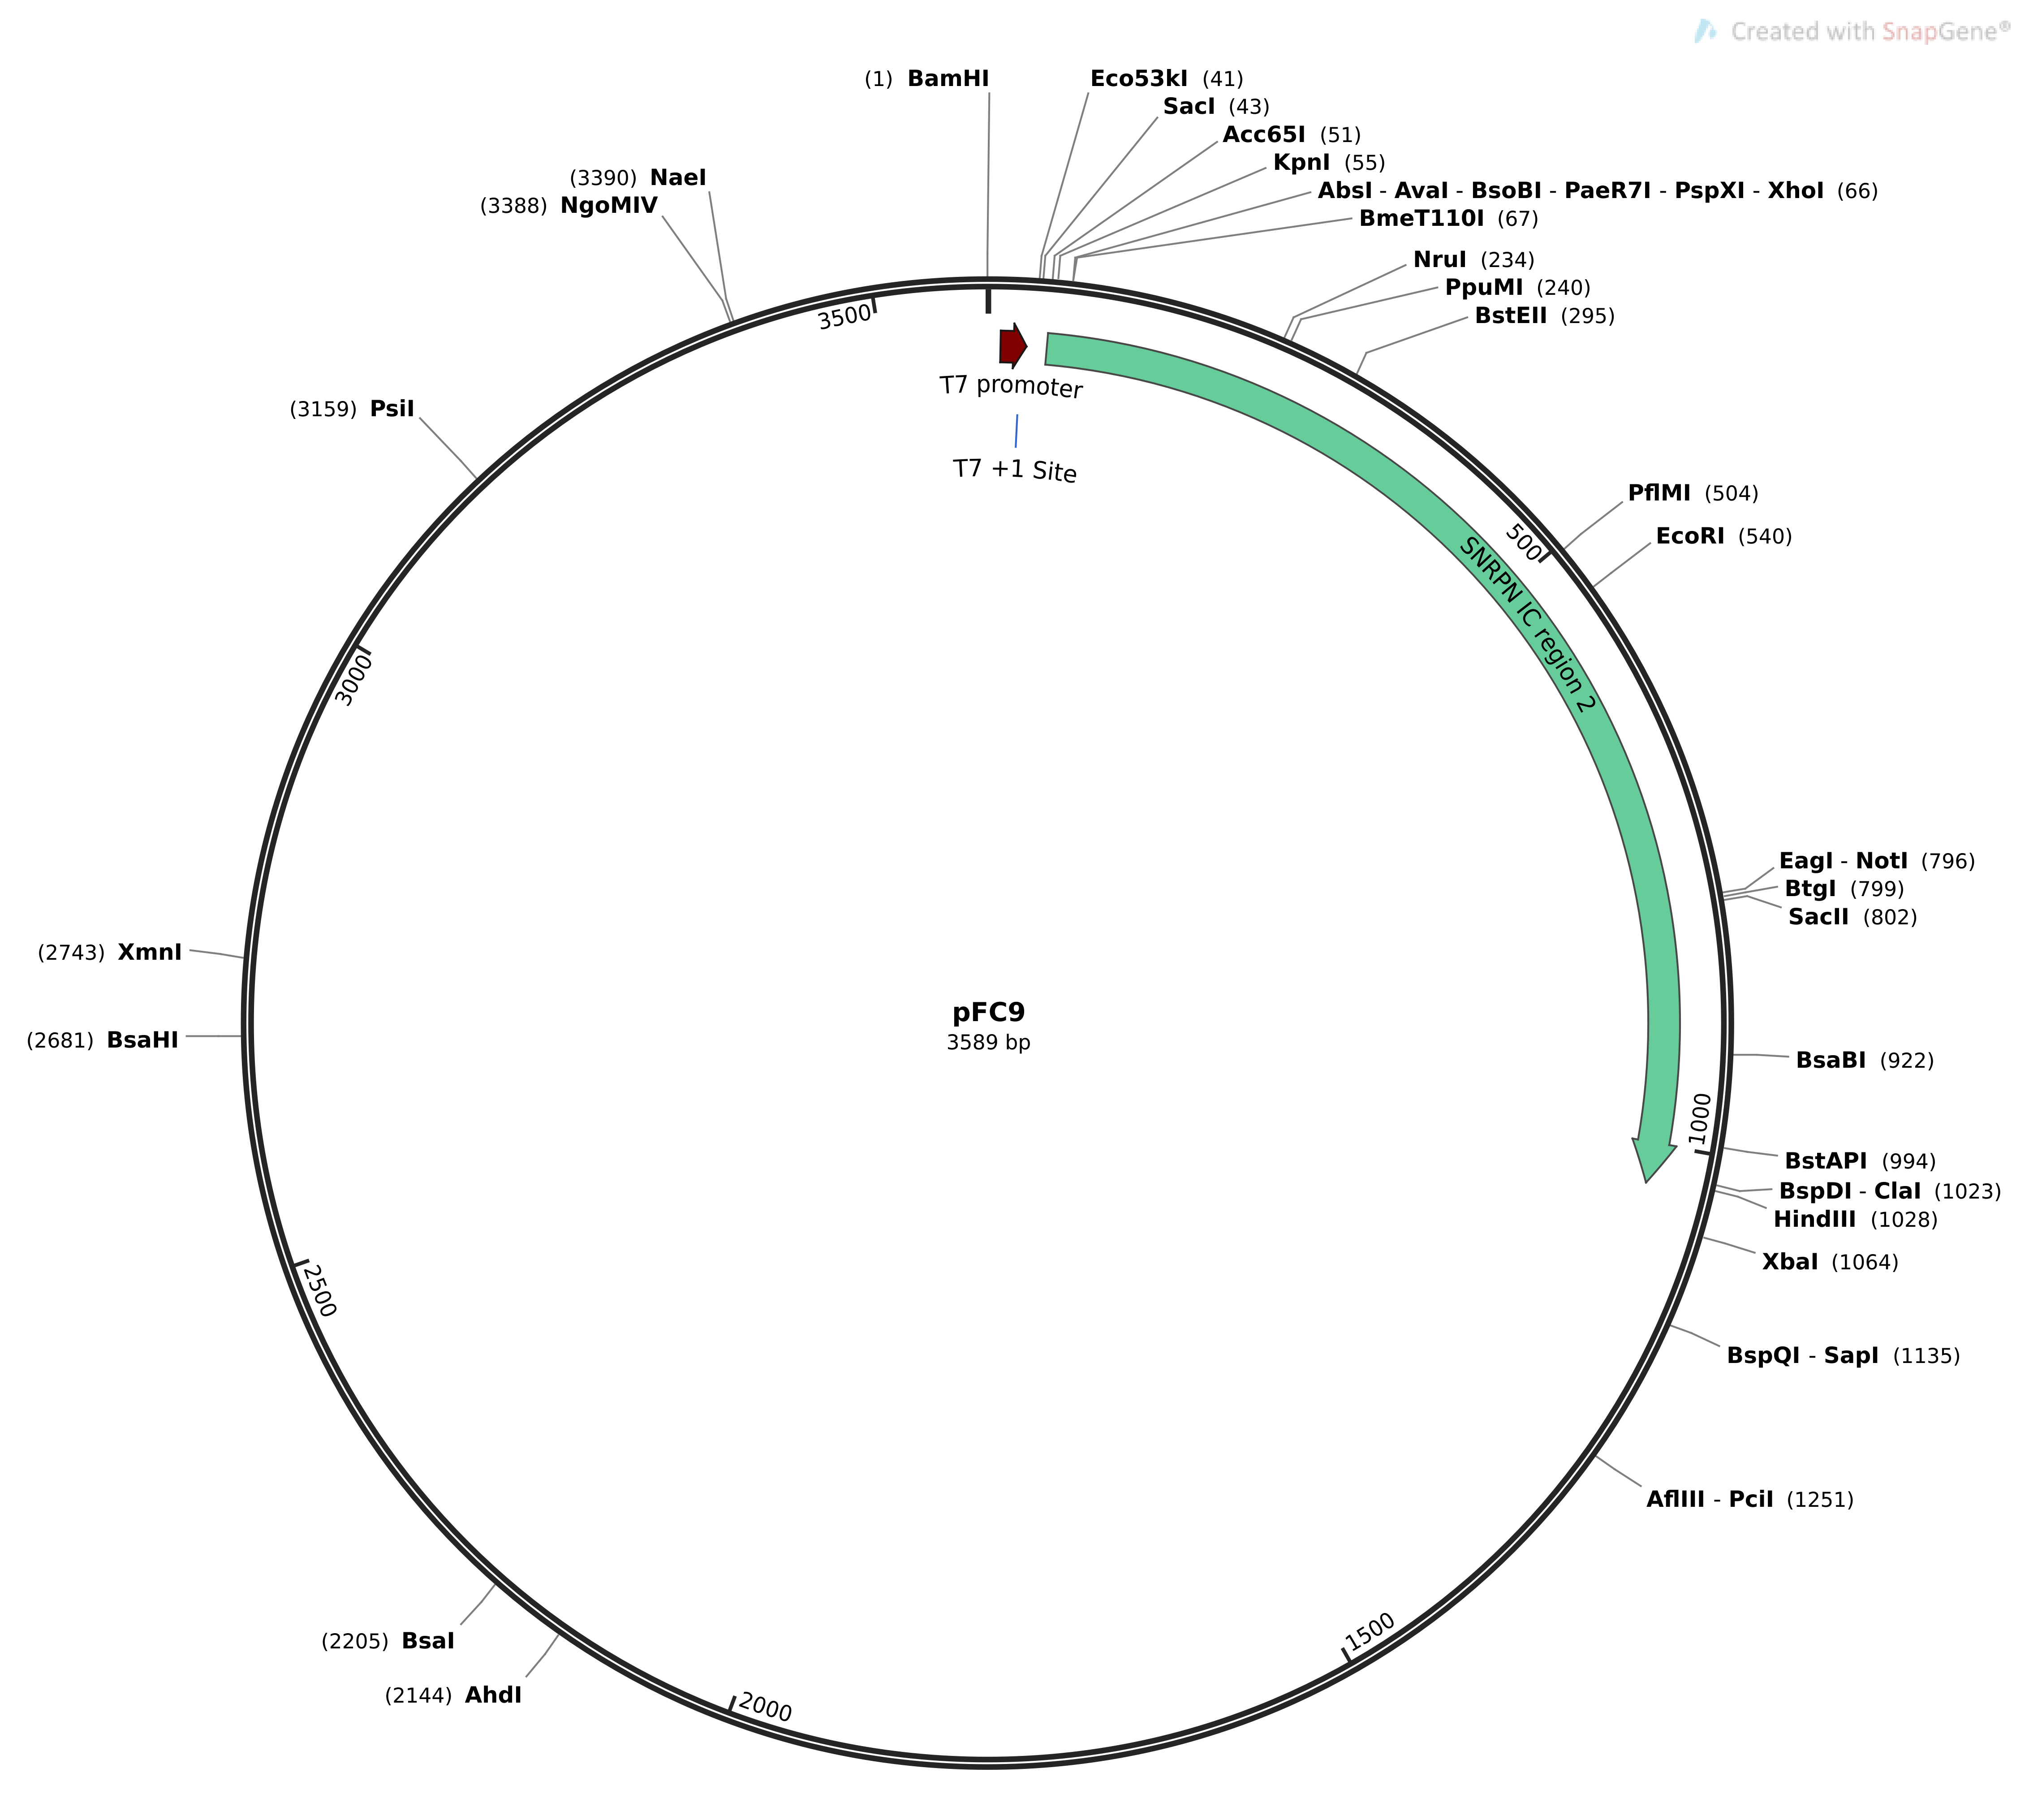
\includegraphics[width=8cm]{images/plasmid_maps/pFC9_Map.png}
	\centering
	\caption{Map of pFC9.}
	\label{fig:map_pFC9}
\end{figure}


\begin{figure}[H]
	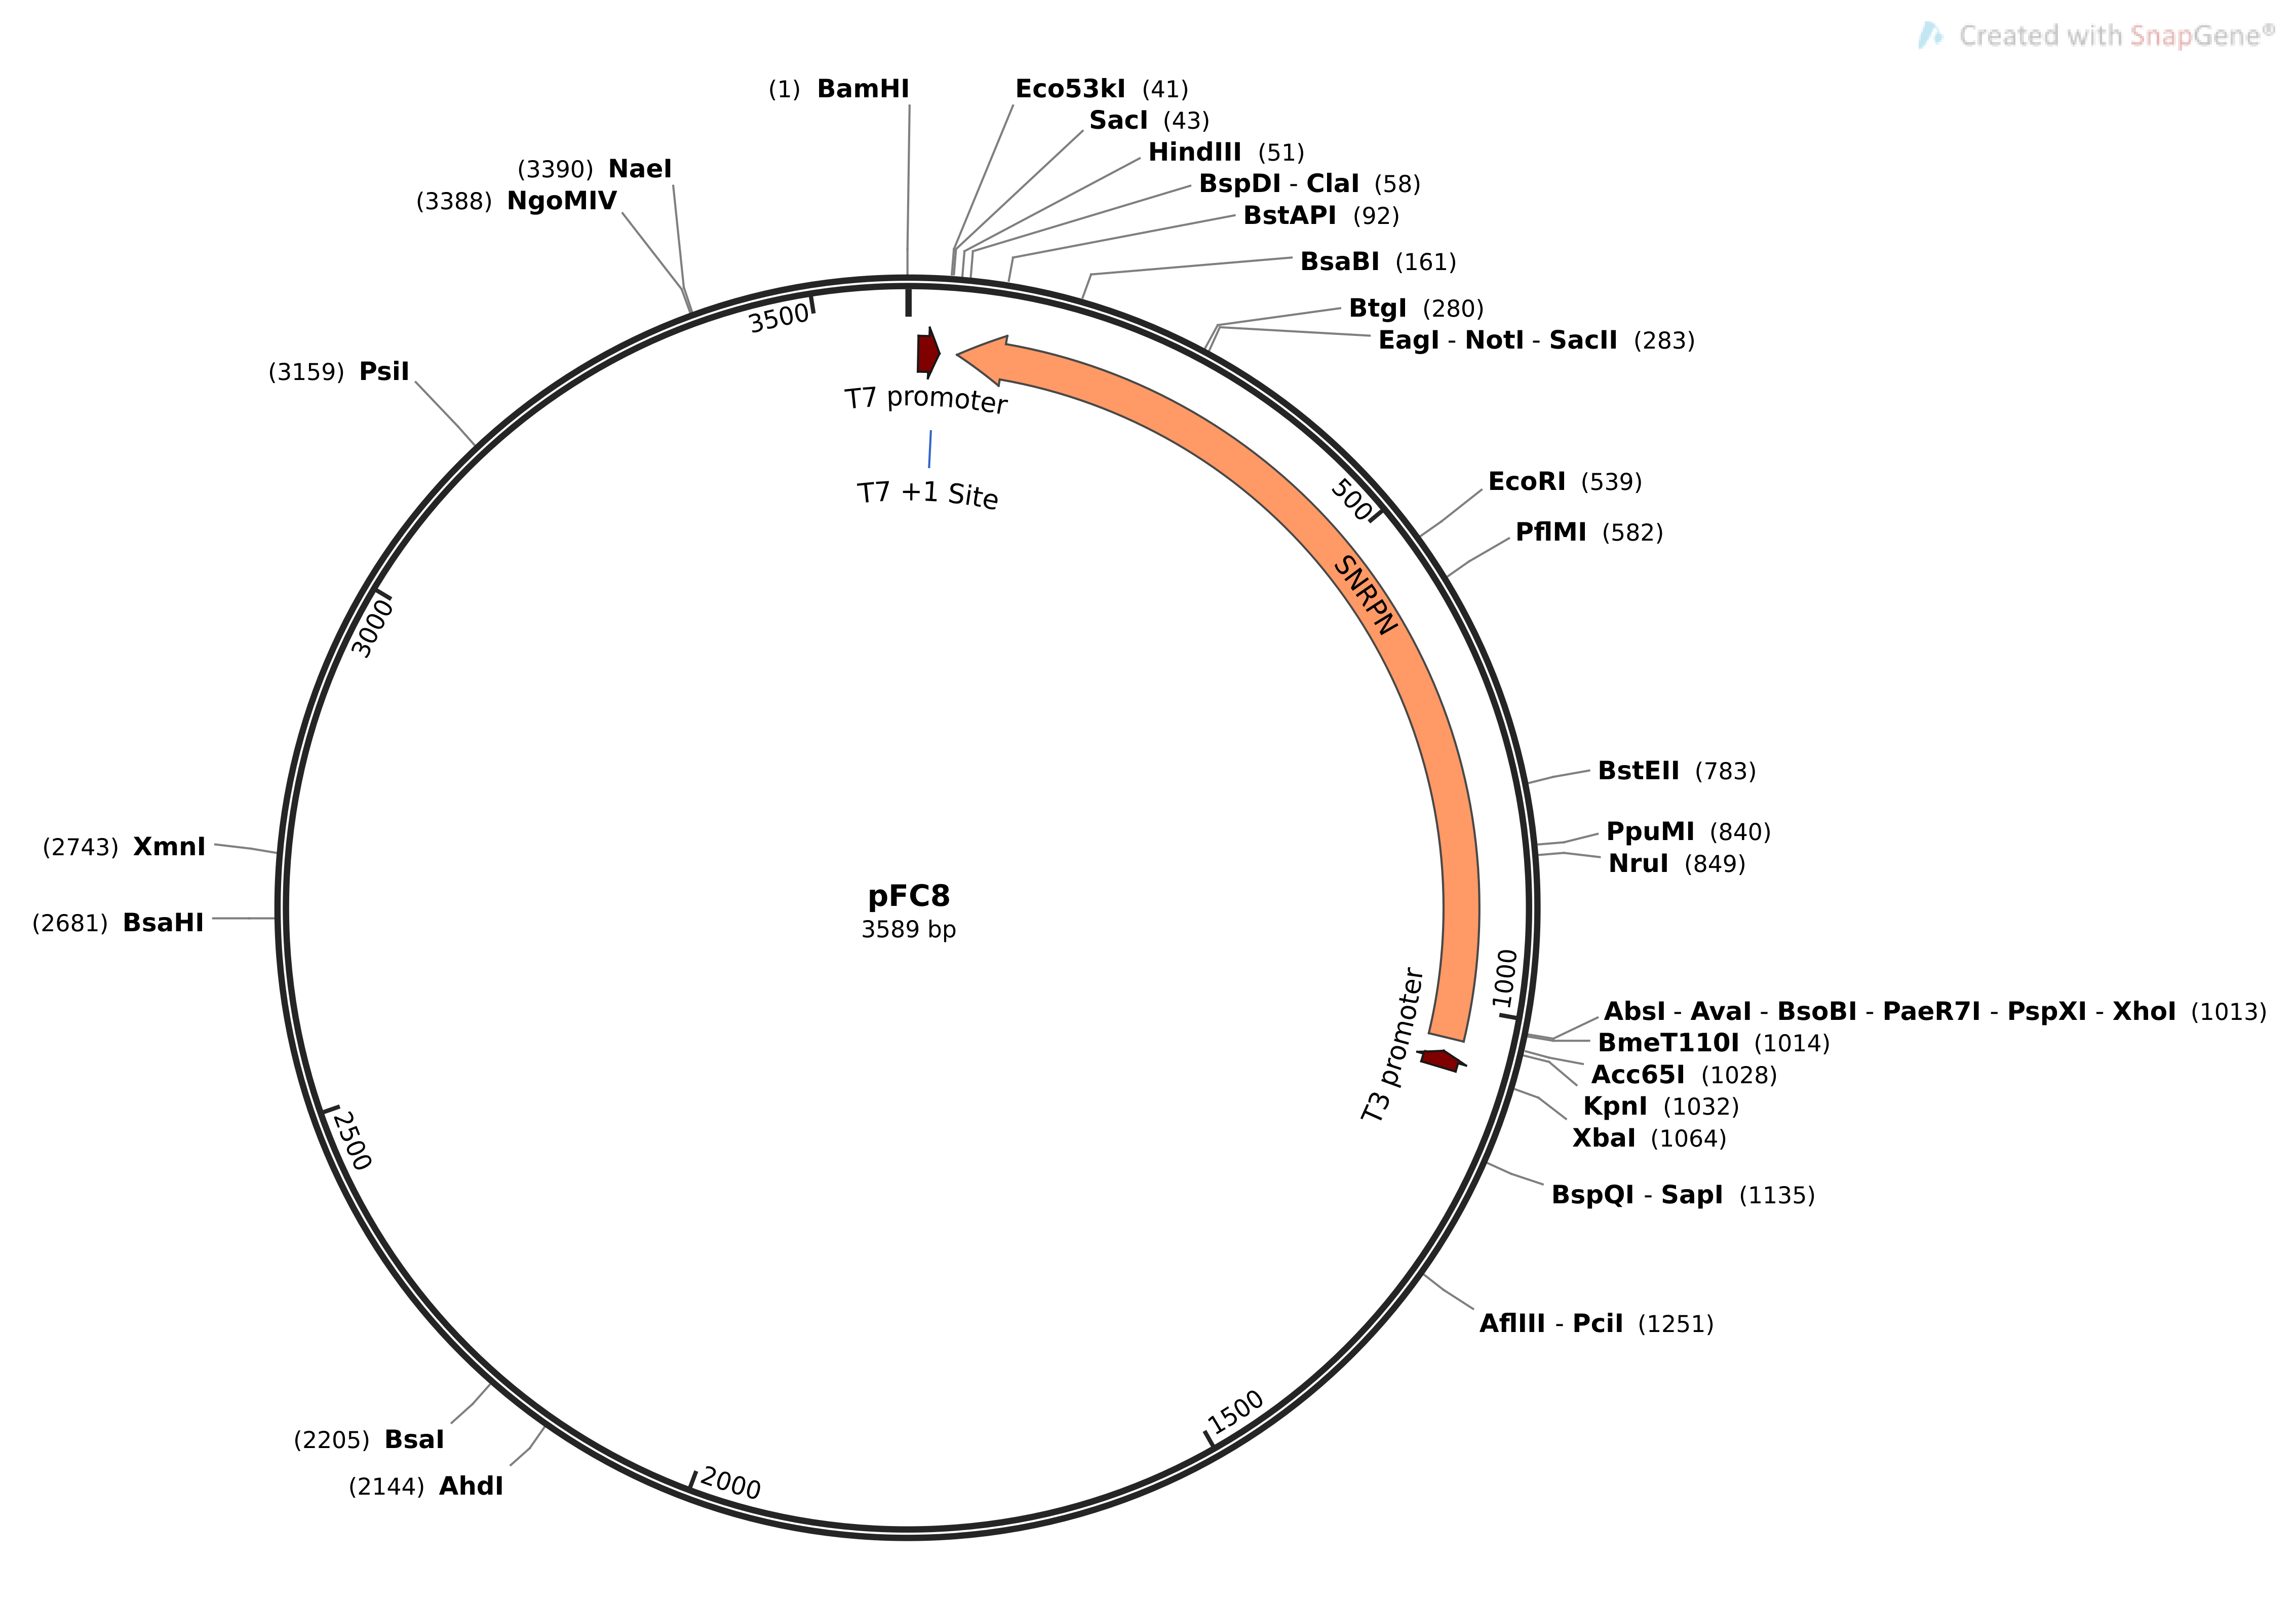
\includegraphics[width=11cm]{images/plasmid_maps/pFC8_Map.png}
	\centering
	\caption{Map of pFC8.}
	\label{fig:map_pFC8}
\end{figure}


\begin{figure}[H]
	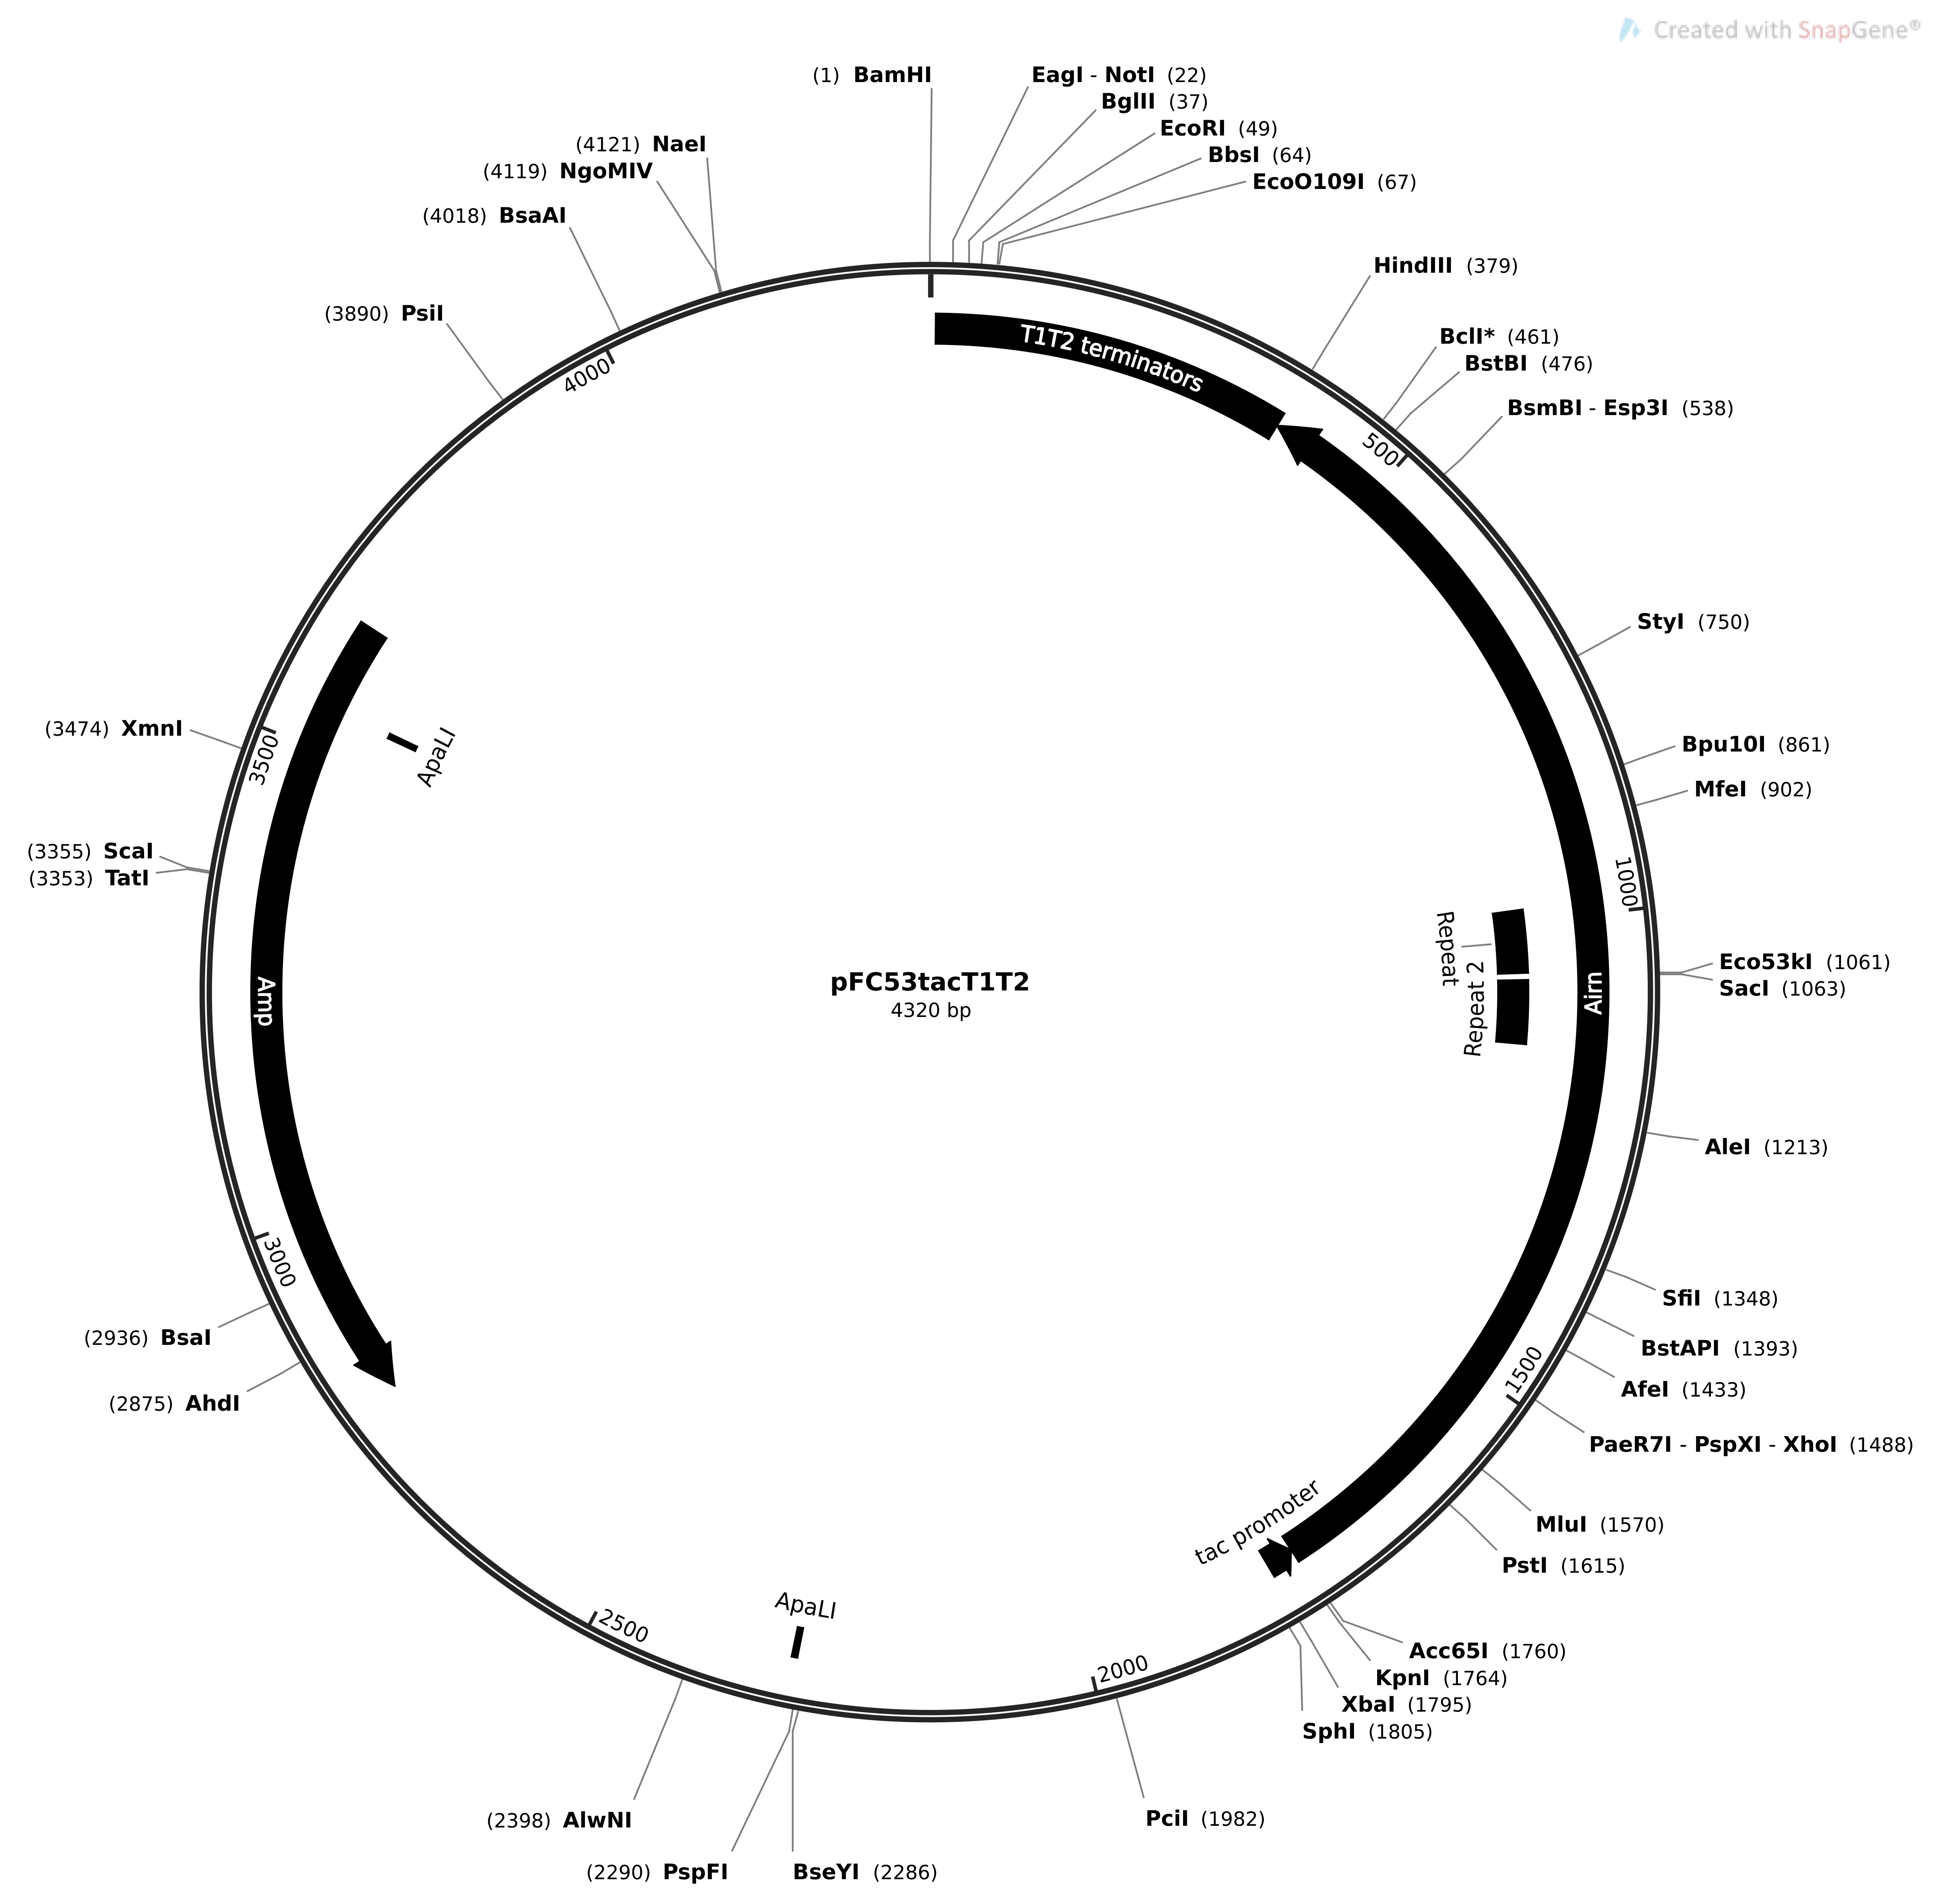
\includegraphics[width=8cm]{images/plasmid_maps/pFC53tacT1T2_Map.png}
	\centering
	\caption{Map of pFC53tacT$_1$T$_2$.}
	\label{fig:map_pFC53tacT1T2}
\end{figure}




\subsection{T7 initiation series constructs}
\label{T7:init} 


\begin{figure}[H]
	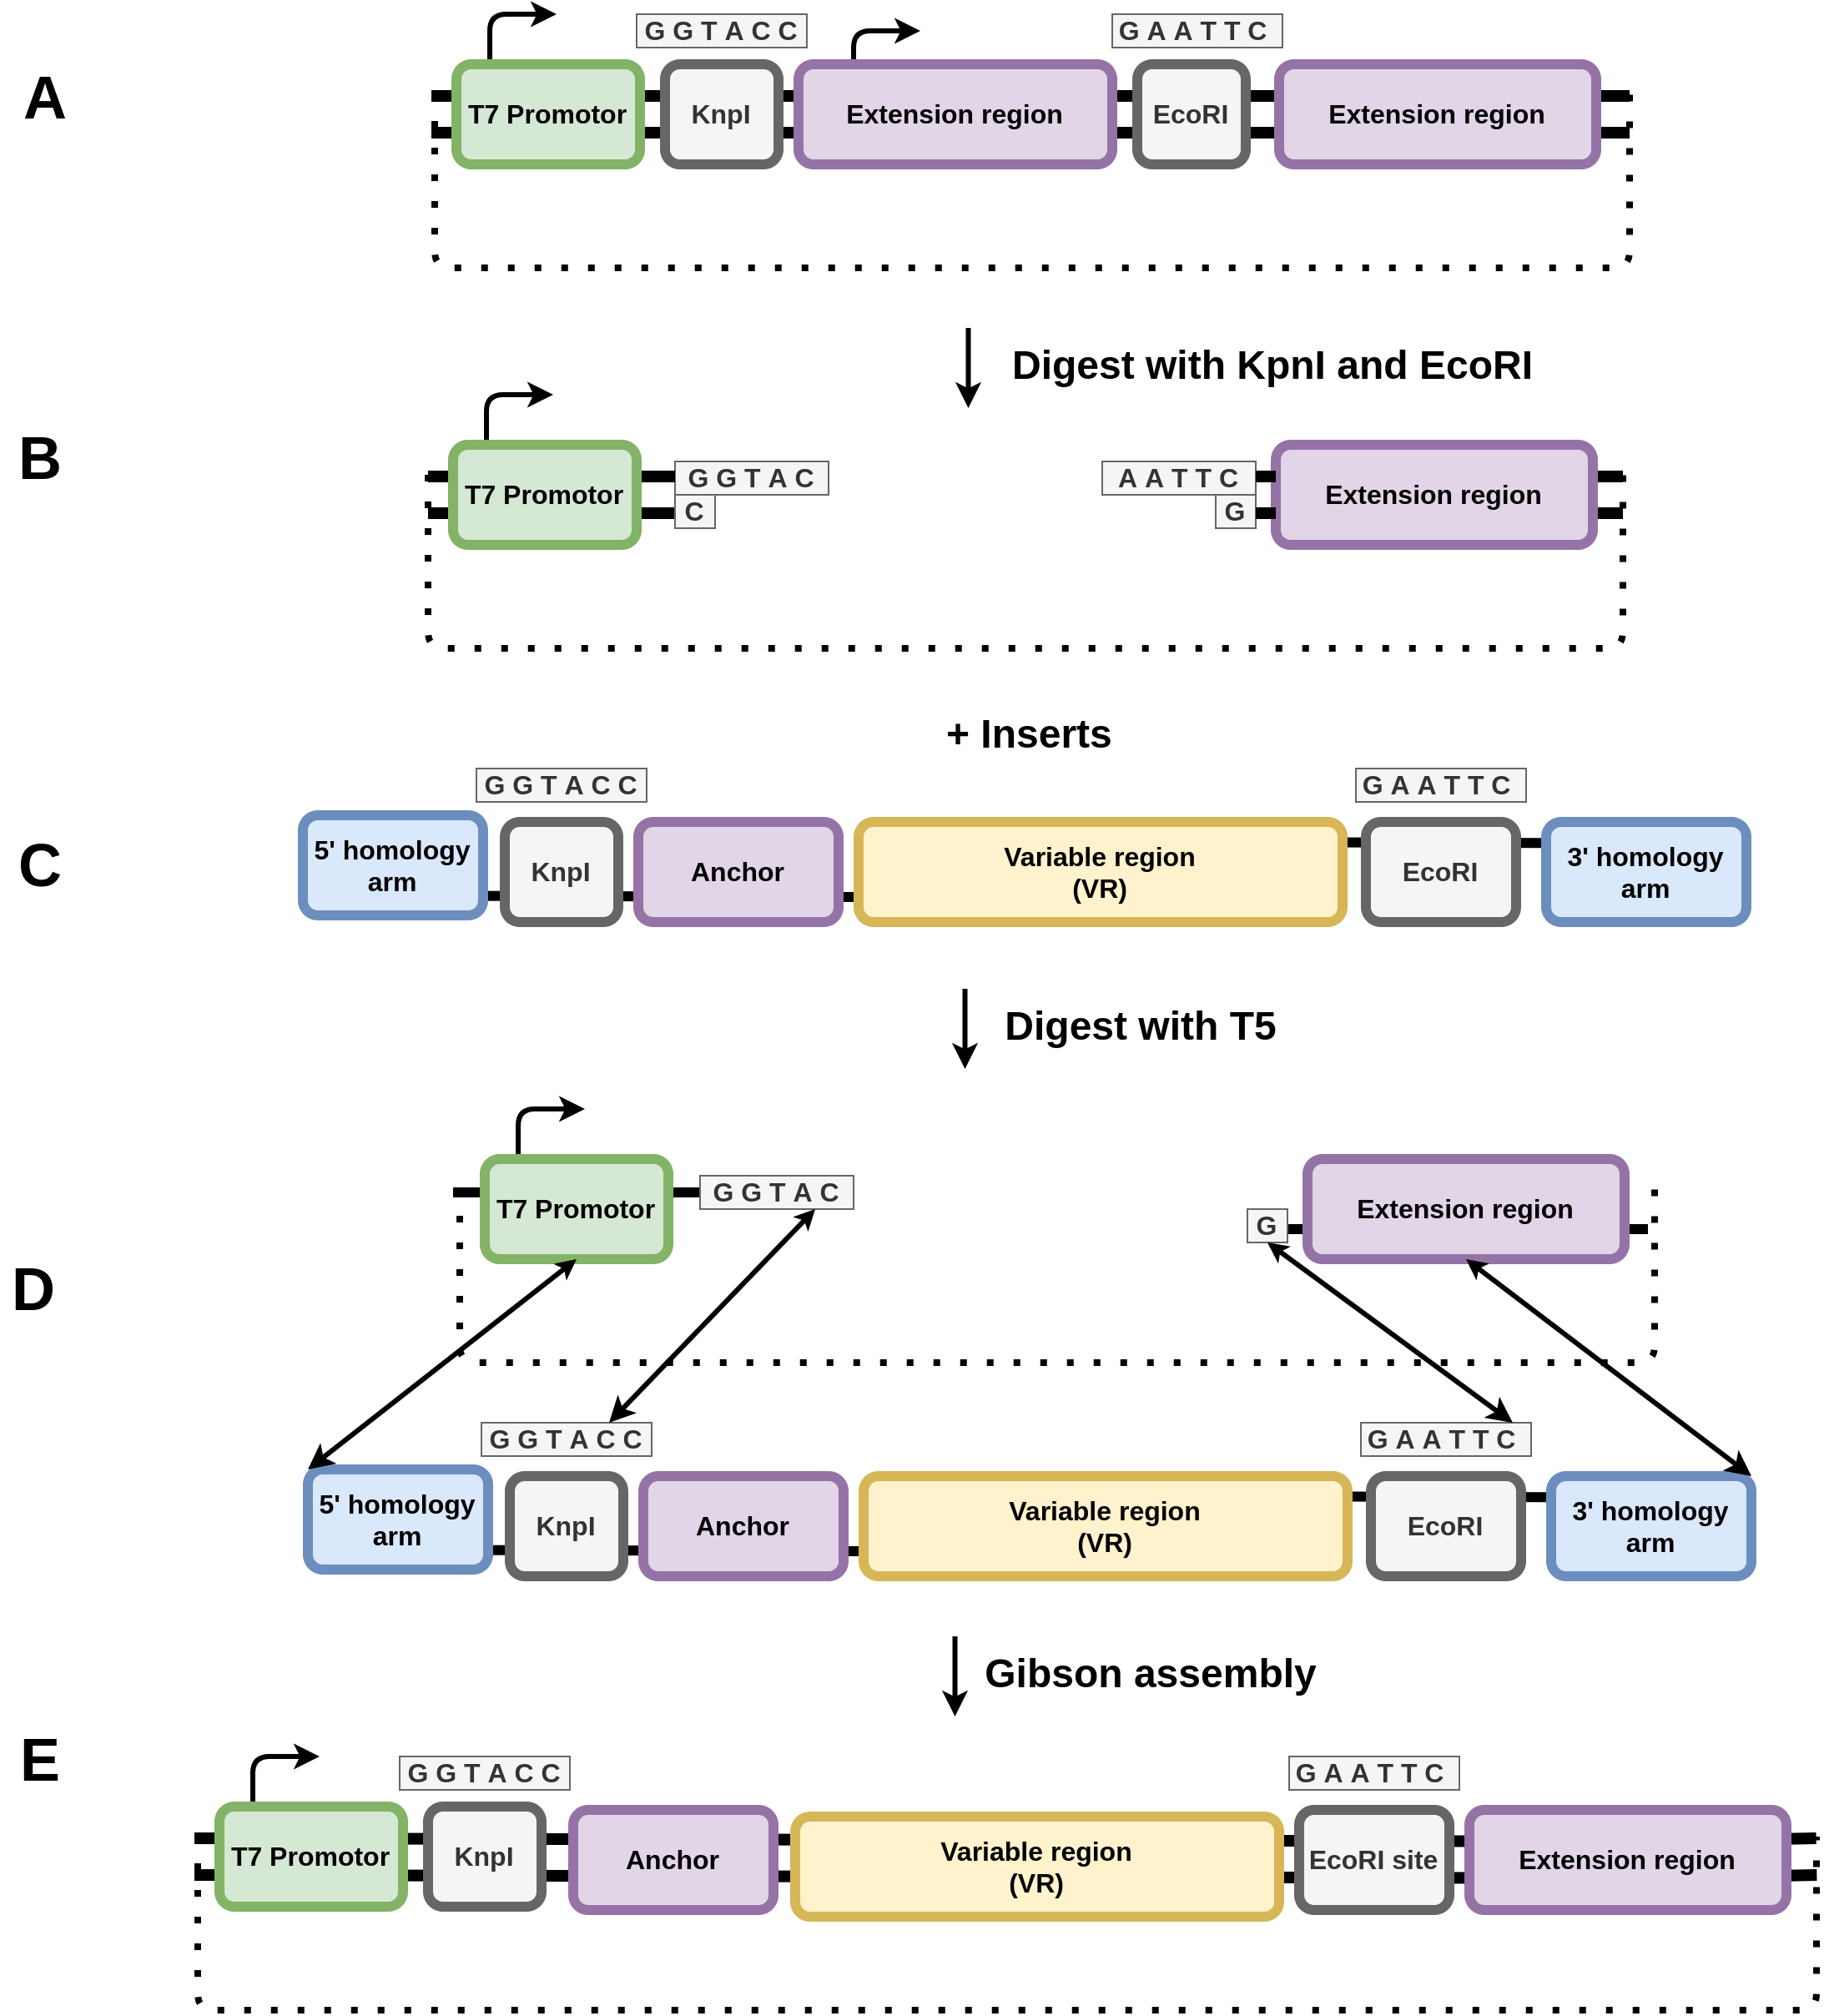
\includegraphics[width=15cm]{images/cloning_diagrams/construct_diagrams-T7-Initiation-series.png}
	\centering
	\caption{Diagram of pFC9 insertion series cloning strategy.}
	\label{clone:T7-insert}
\end{figure}

First, pFC9 will be linearized by digestion with KpnI and EcoRI  (fig \ref{clone:T7-insert}A). The large pFC9 fragment will then be purified and added to a mixture containing all insert sequences in equal concentration  (fig \ref{clone:T7-insert}B). Next, T5 exonuclease is added to digest the 5' ends of all DNA in the mixture. This will leave the 3' overhang of the digested KpnI site intact but degrade the 5' overhang of EcoRI  (fig \ref{clone:T7-insert}C). The 5' ends of the insert will also be degraded exposing exposing the complete KnpI and EcoRI sites present in each insert. Next, during Gibson assembly the 5' homology arm and KnpI site will anneal to the pFC9 large fragment, overhanging the digested KnpI site by 1 nucleotide; a C. Similarly, the 3' homology arm and intact EcoRI site of the inserts will anneal to the pFC9 large fragment, with only the last nucleotide (C) of the insert's intact EcoRI site annealing to the 3' G present at the digested EcoRI site of the pFC9 large fragment (fig \ref{clone:T7-insert}D). This will result in a library of circular constructs with all inserts located downstream of and oriented forward relative to, the pFC9 T7 promoter (fig \ref{clone:T7-insert}). 


\subsection{T7 termination series constructs}

After the successful sequencing of the T7 initiation series, pFC8 will be utilized as the backbone for construction of the termination series library. 

\begin{figure}[H]
	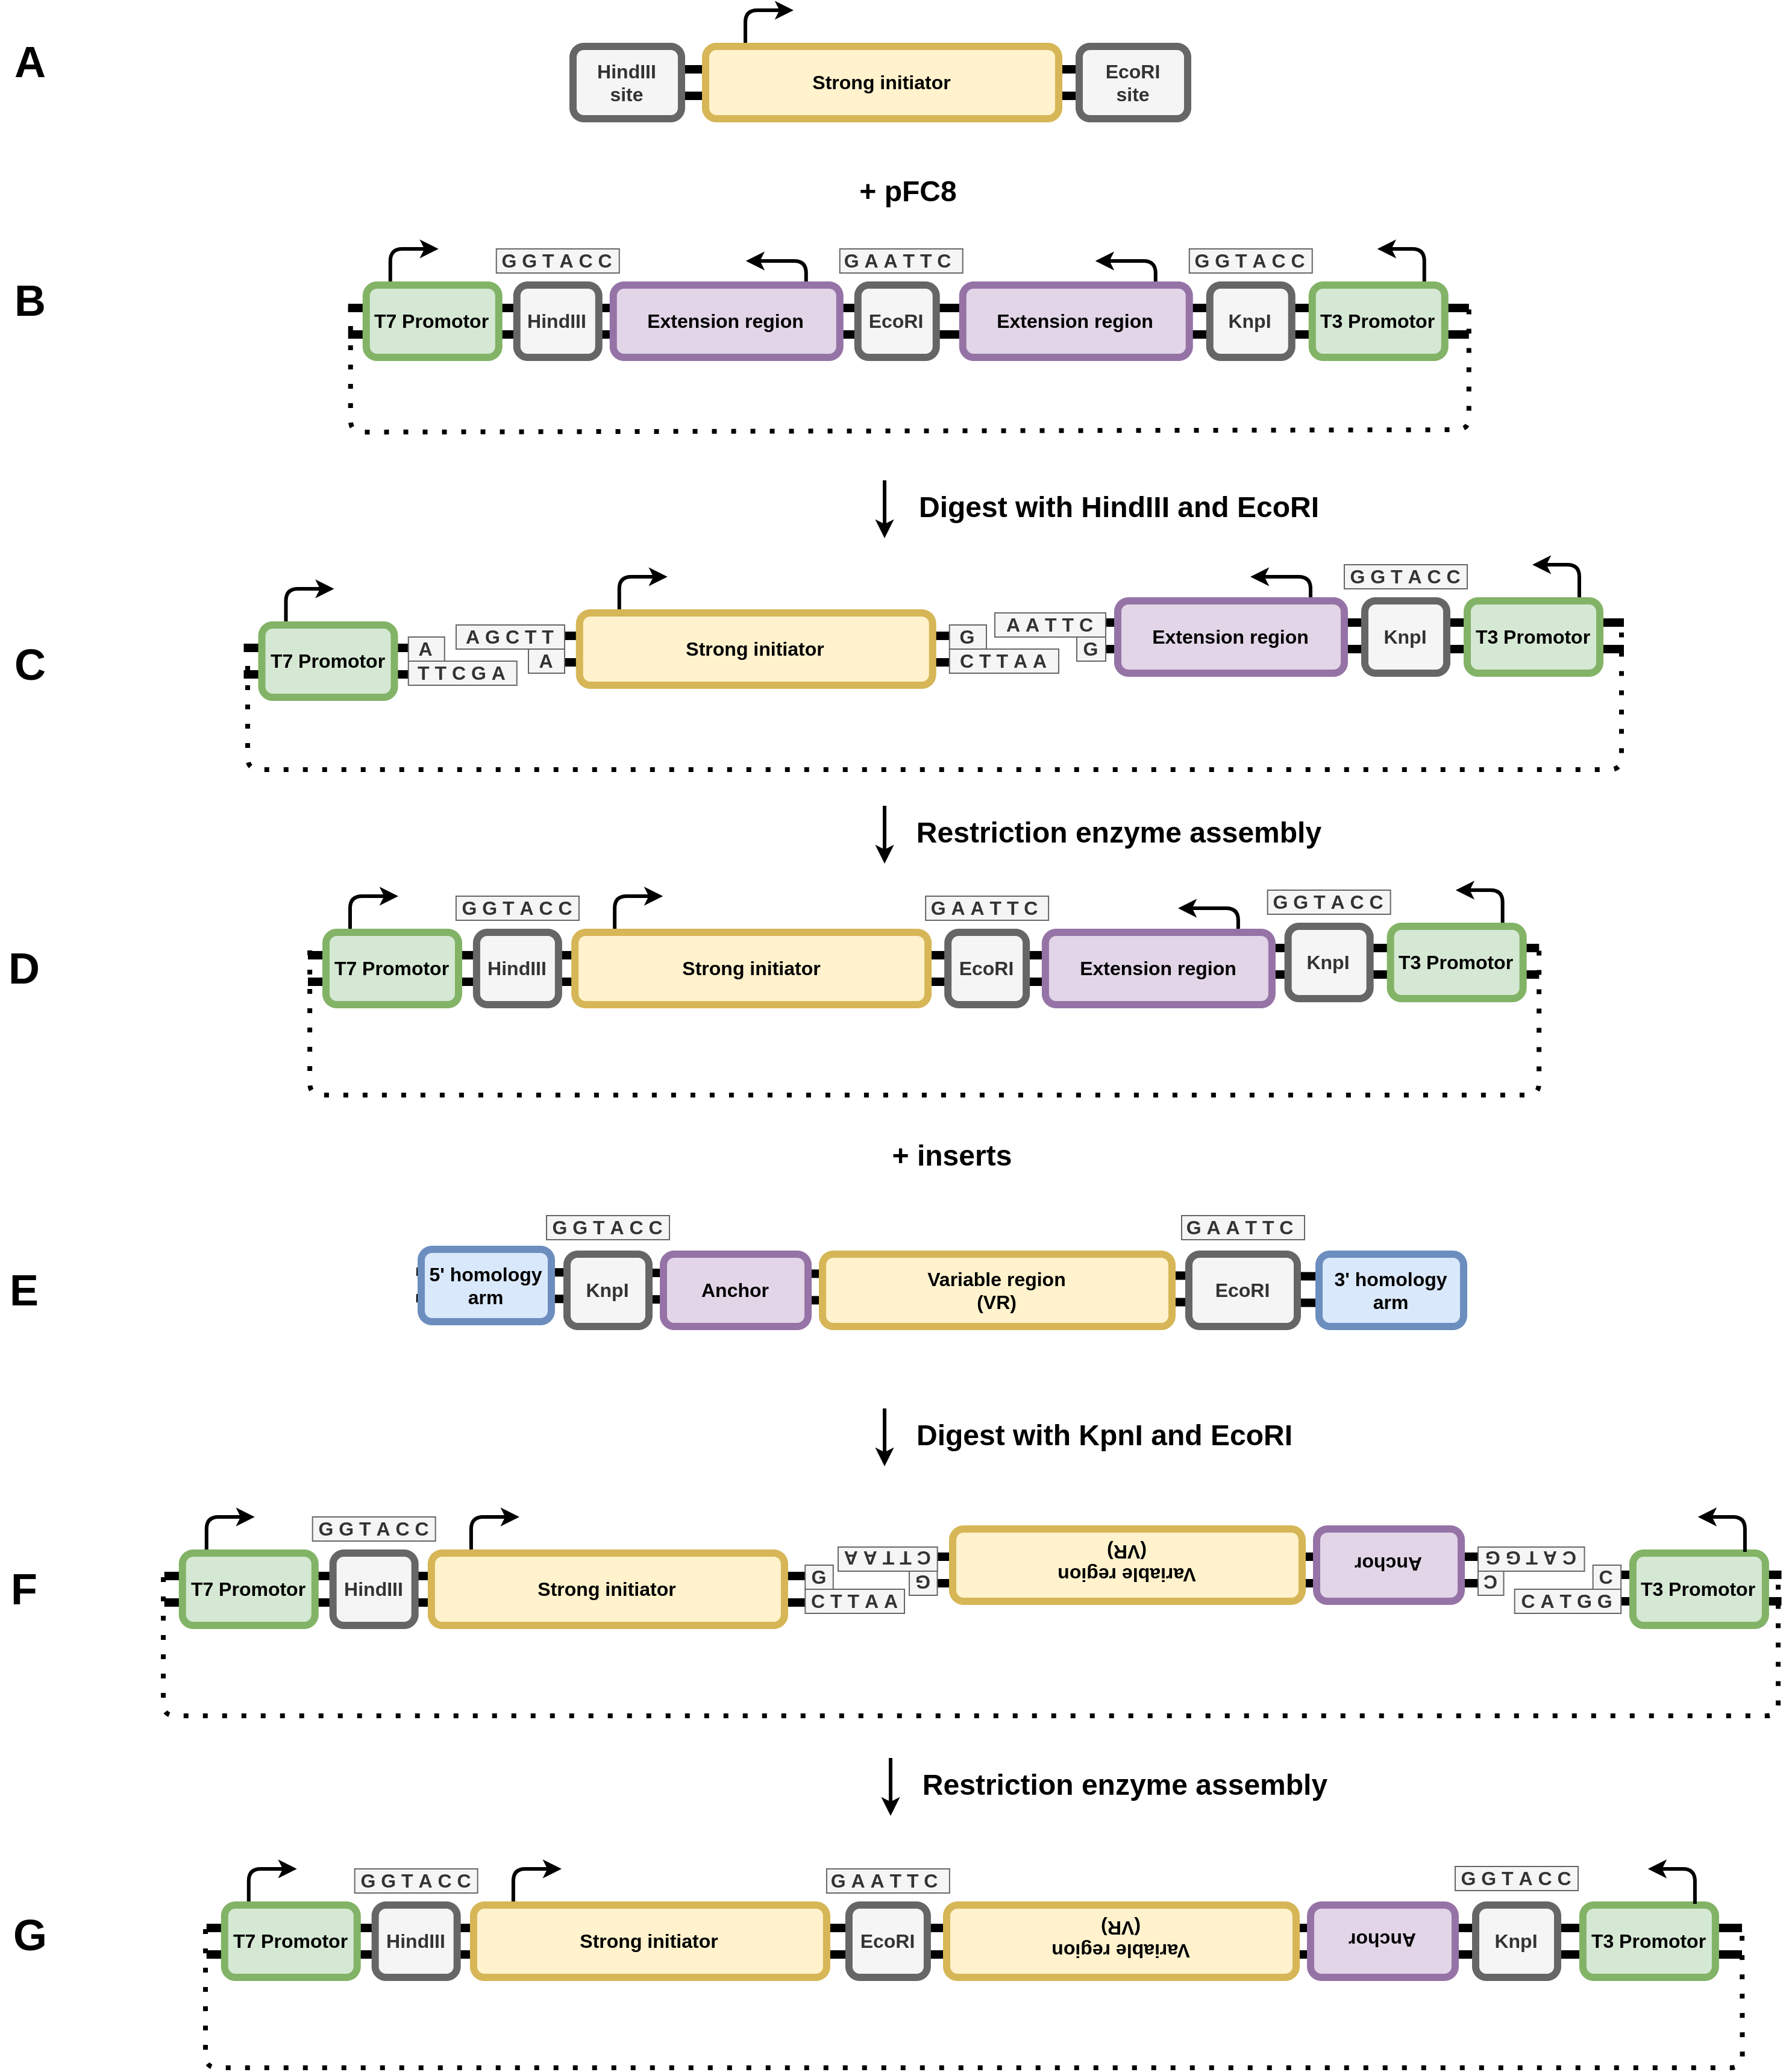
\includegraphics[width=15cm]{images/cloning_diagrams/construct_diagrams-T7-termination-series.png}
	\centering
	\caption{Diagram of pFC9 insertion series cloning strategy.}
	\label{clone:T7-term}
	
\end{figure}

 First, the strongest and most consistent R-loop initiator identified from the T7 initiation series will serve as the substrate for an additional synthetic double stranded DNA fragment containing the strong initiator sequence flanked by  HindIII and EcoRI recognition sequences (\ref{clone:T7-term}A). This strong initiator fragment will be added to pFC8  (\ref{clone:T7-term}B) and then the mixture digested with HindIII and EcoRI. The strong initiator will then anneal to the large pFC8 fragment via homology between the digested HindIII and EcoRI recognition sites (\ref{clone:T7-term}C). Next all termination inserts will be added to the pFC8-strong-initiator construct in equal concentrations (\ref{clone:T7-term}D) and the mixture digested with KpnI and EcoRI (\ref{clone:T7-term}E). Inserts will then be incorporated into pFC8-strong-initiator constructs via homology between the digested KpnI and EcoRI sites (\ref{clone:T7-term}F). Since the order of these recognition sites on the pFC8-strong-initiator construct is opposite to that of the insert with respect to the T7 promoter the inserts will be present in the final construct in the reverse orientation and place the variable region downstream of the strong initiator (\ref{clone:T7-term}G). 
 

\subsection{Tac initiation series constructs}
\label{sec:tac-init}


\begin{figure}[H]
	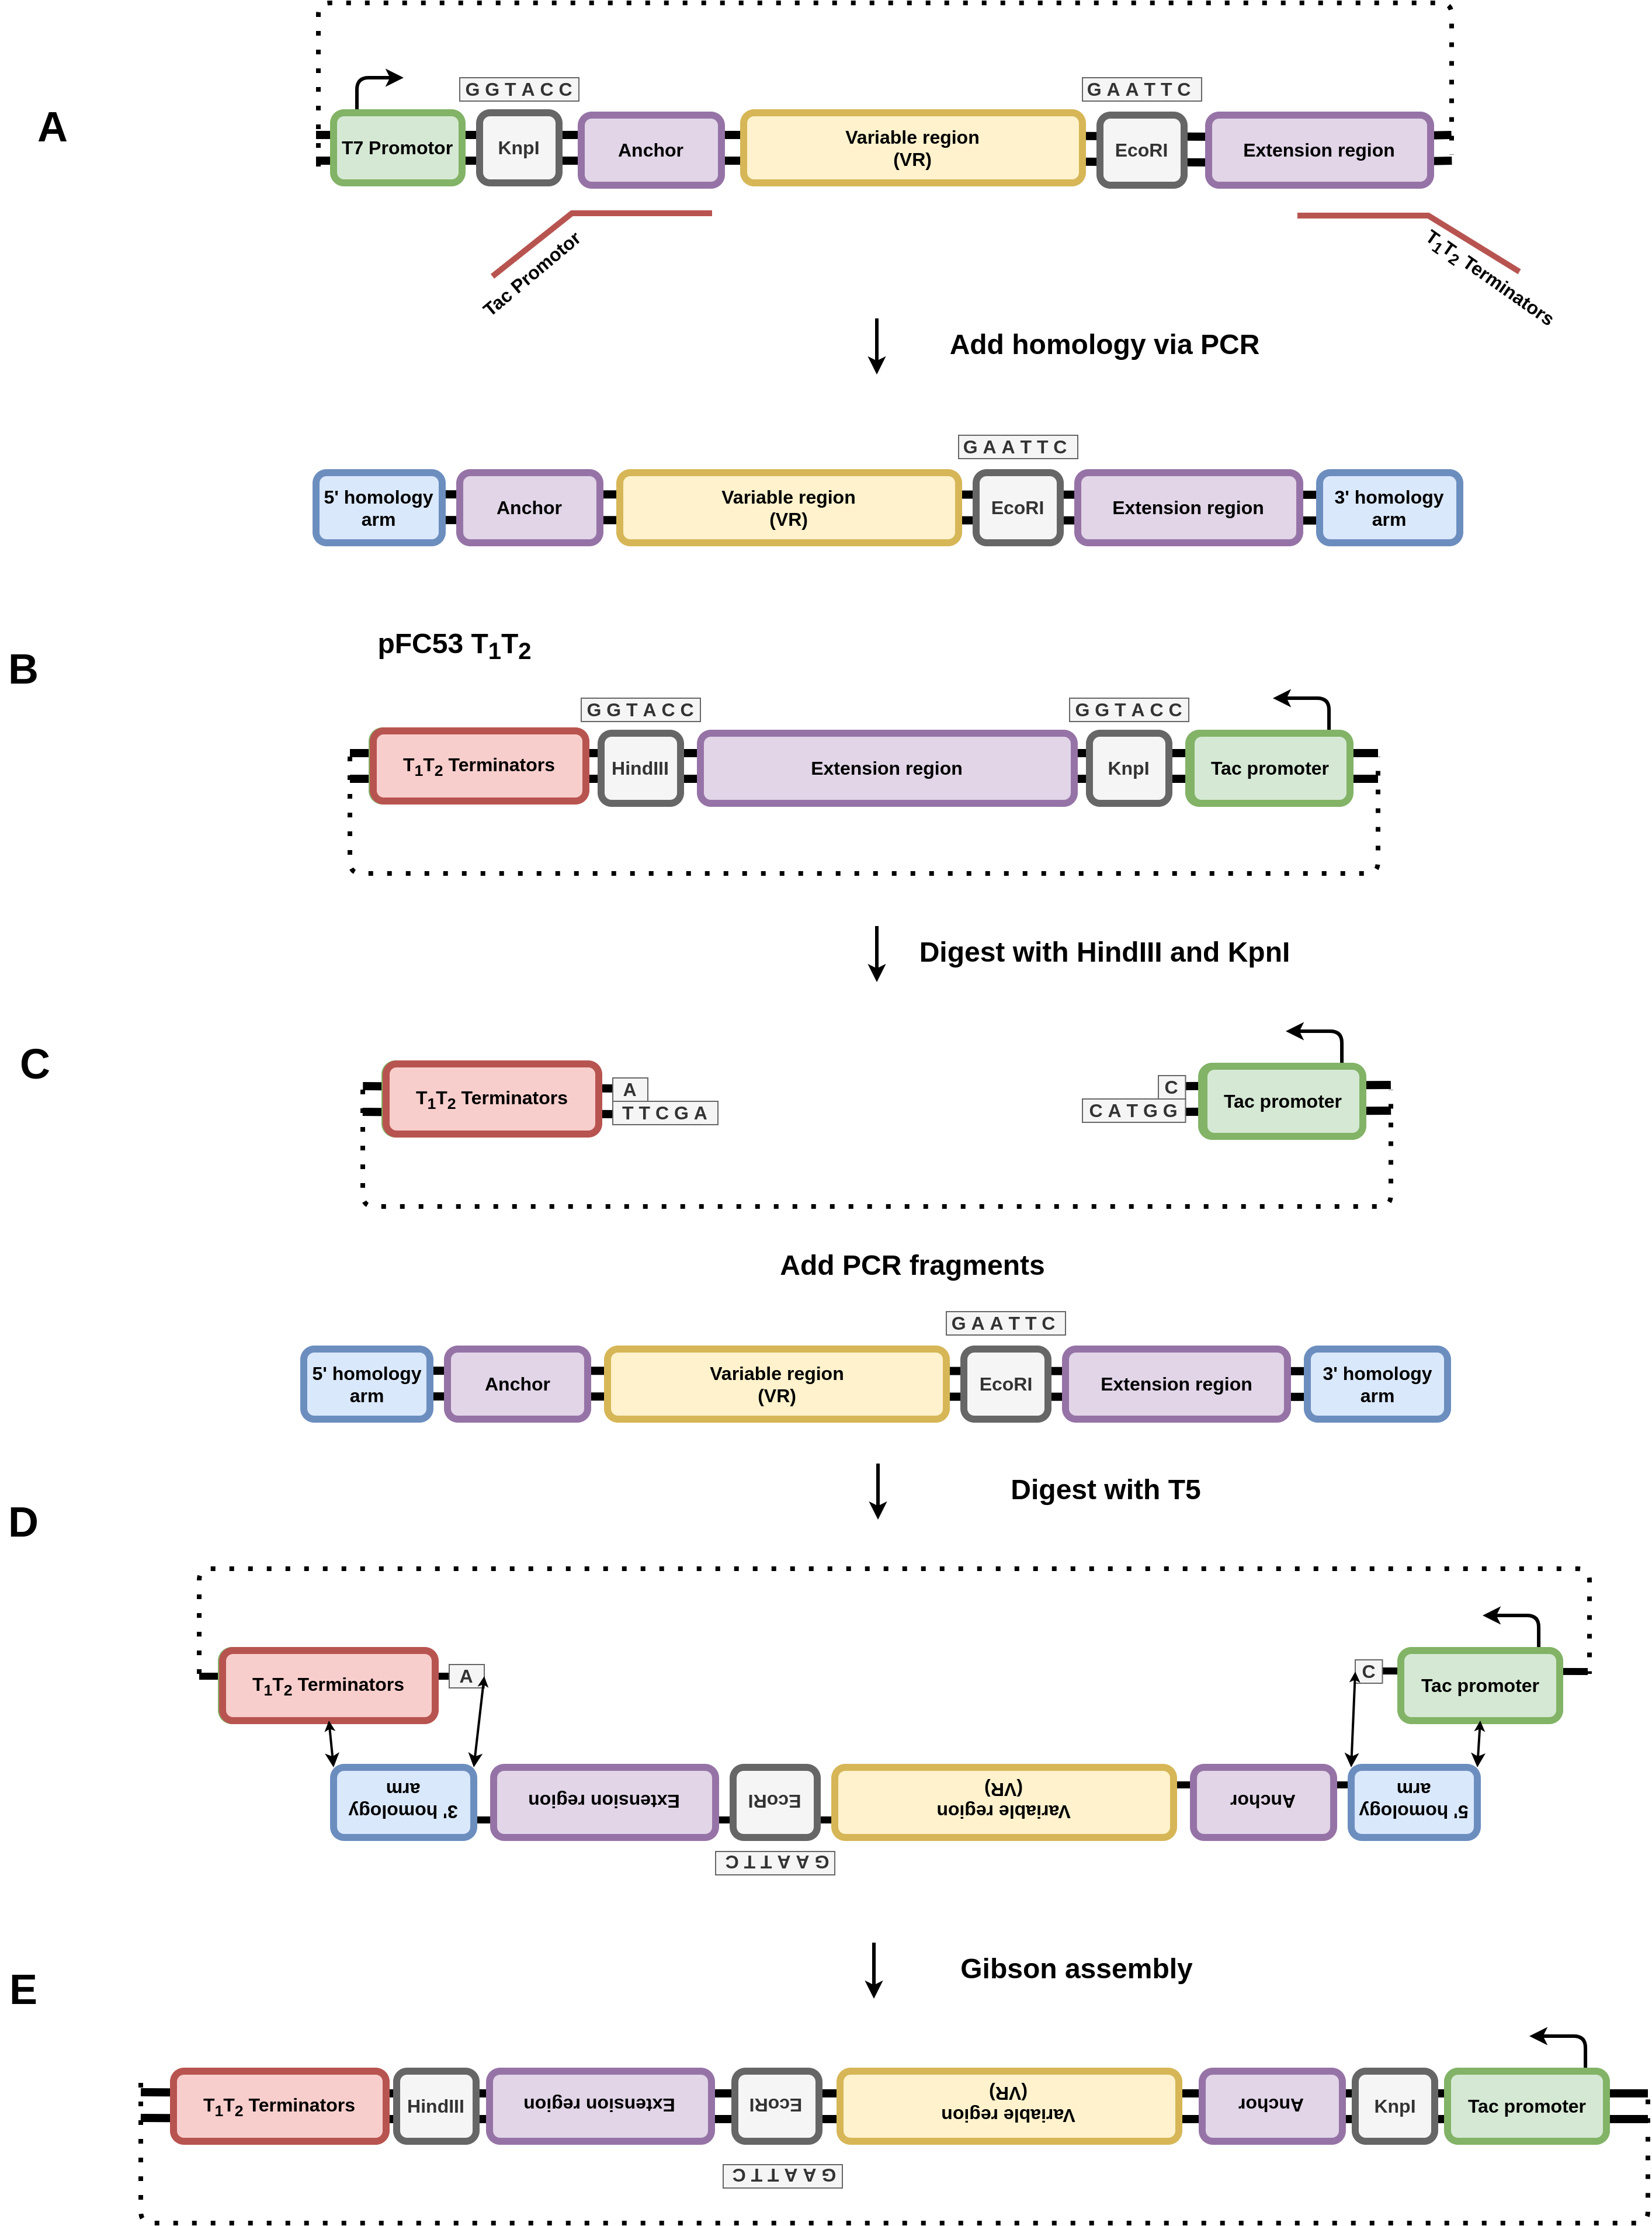
\includegraphics[width=15cm]{images/cloning_diagrams/construct_diagrams-Tac-initiation-series.png}
	\centering
	\caption{Diagram of pFC9 insertion series cloning strategy.}
\end{figure}

First primers two pairs of primers are used to add amplify the anchor region, variable region, EcoRI recognition site and extension region from the T7 initiation construct library (\ref{sec:tac-init}). These primers will also contain 15 bp overhangs with homology to the 5' end of the tac promoter and 3' T1T2 terminator sequences. Next, the PCR products are added to pFC53T1T2 

\subsubsection{Tac initiation series primer design}

\subsection{Tac termination series constructs}
\label{sec:tac-termination}


\begin{figure}[H]
	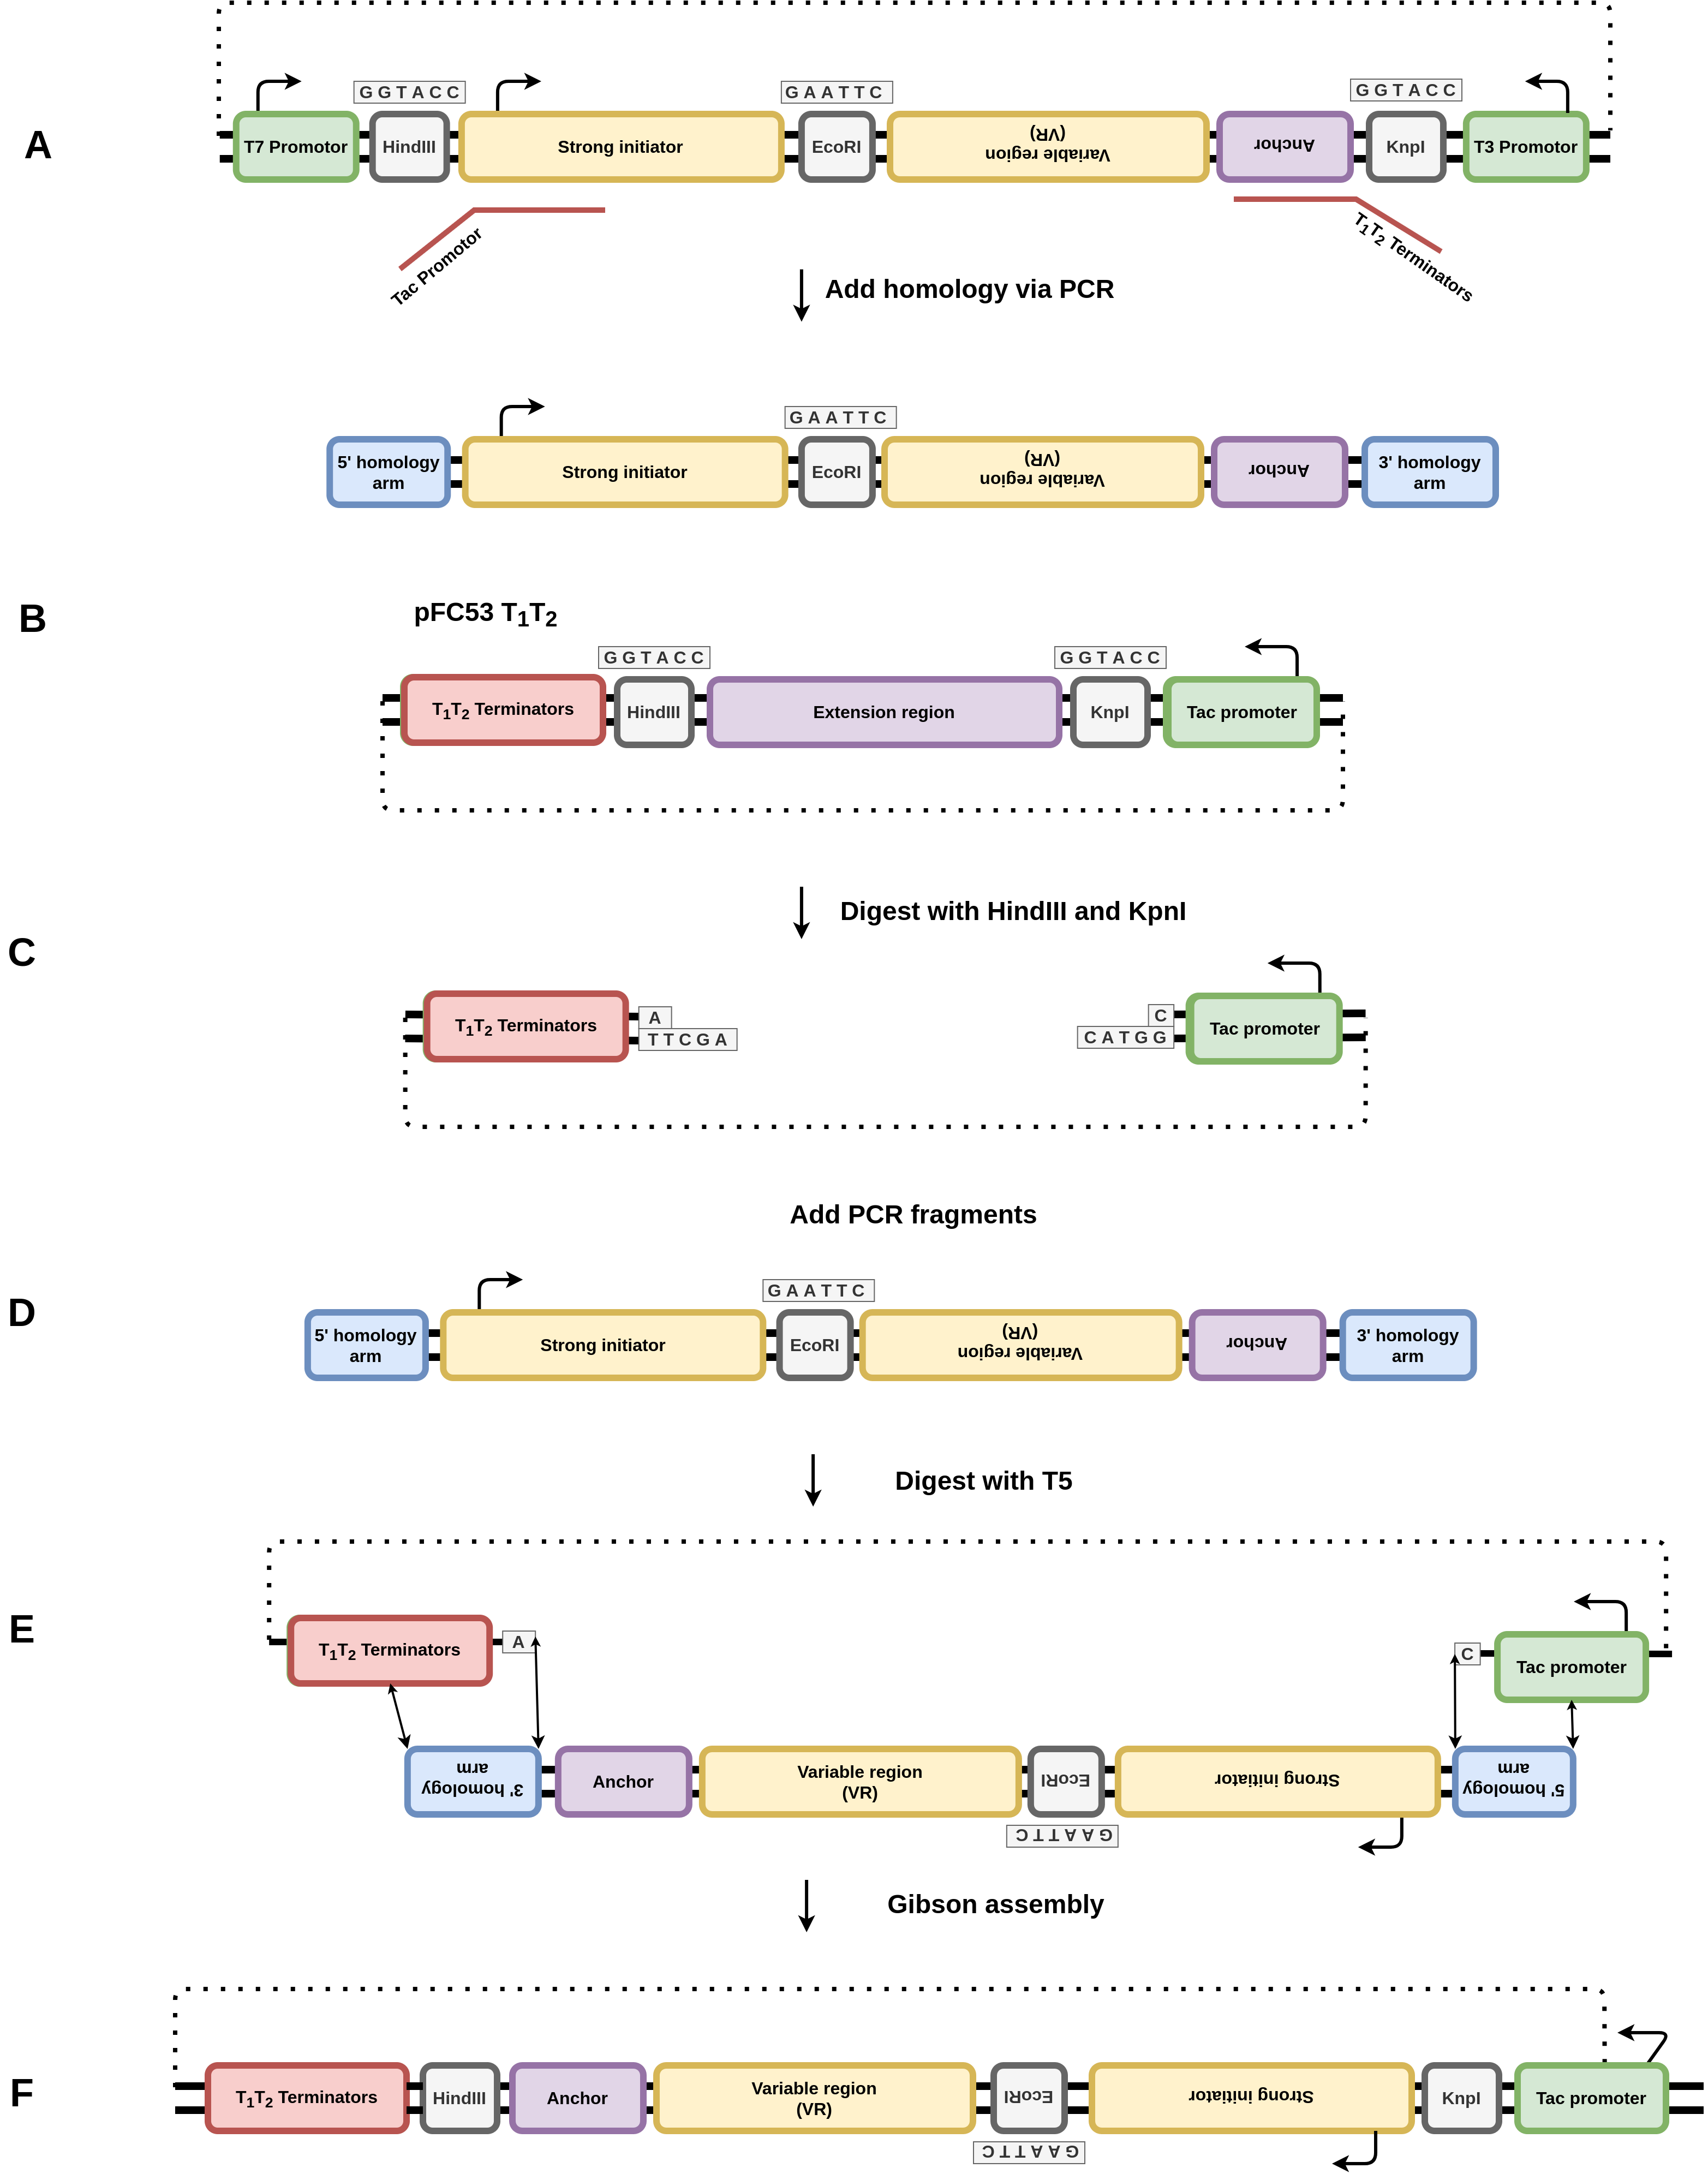
\includegraphics[width=15cm]{images/cloning_diagrams/construct_diagrams-Tac-termination-series.png}
	\centering
	\caption{Diagram of pFC9 insertion series cloning strategy.}
\end{figure}

\subsubsection{Tac termination series primer design}

\subsection{Validation of insert libraries}

Use qPCR with primers for subset of variable regions with divergent characteristics should be present in equal quantities or just use primers for everything but then need to design unique primers or at least one primer that ends in the variable region so is specific to each insert. 

\subsection{Quantification of R-loop formation }

Short description of SMRF-seq protocol using barcoded PCR primers for amplification 
and anticipated data analysis. 

\section{Sequence availability}

Final versions of all complete insert sequences in fasta and genbank format are available at this link. For convenience, a copy of the fasta formatted file is also included in this document in section \ref{sec:fasta-inserts}. 


\section{Code availability}

All code used in insert creation and analysis is available here. The source code for this document is available at the GitHub repository \href{https://github.com/EthanHolleman/plasmid-VR-design}{at this link}.

\section{Supplementary materials}

\subsection{Variable region snakemake pipeline diagram}

\begin{figure}[H]
	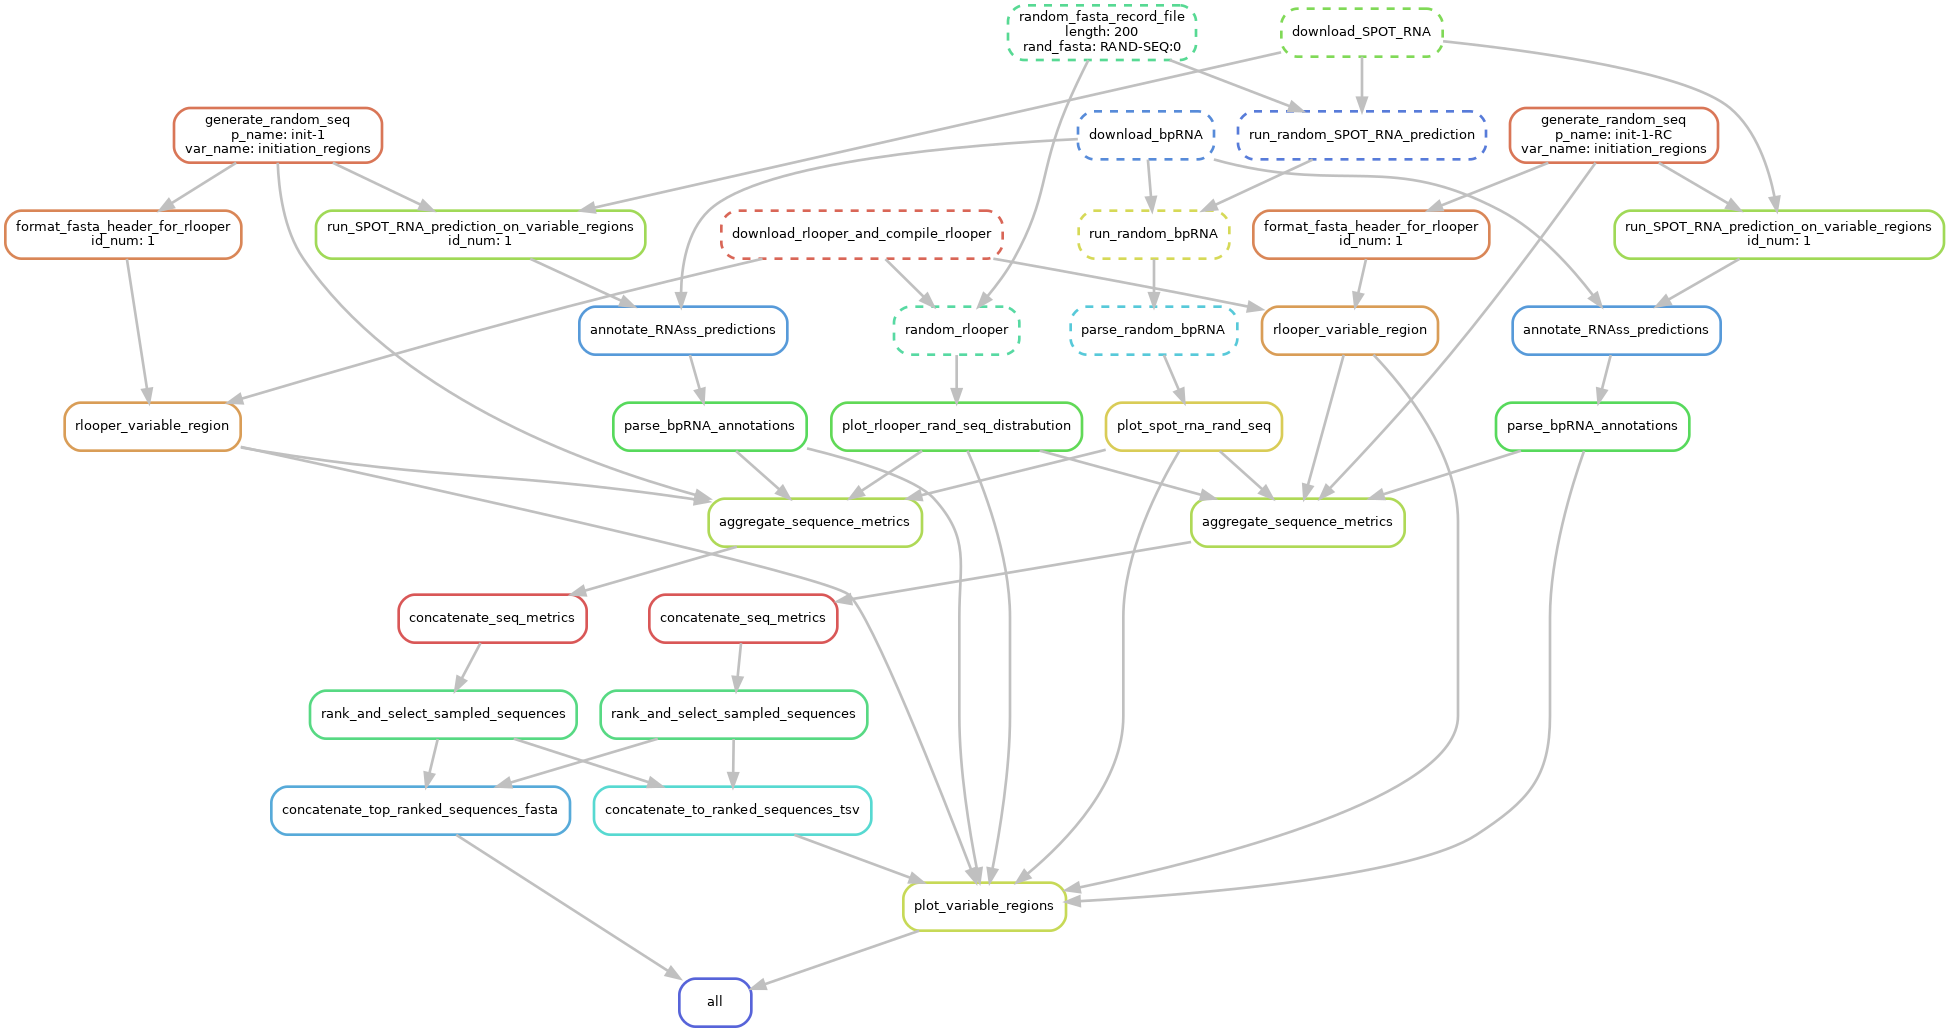
\includegraphics[width=15cm]{images/misc/dag.png}
	\centering
	\caption{Place holder dag image.}
\end{figure}

\subsection{Initial R-looper expectation calculations}

Originally, expectations for R-looper results were derived by measuring average per base pair probability and of R-loop formation average per base pair local average energy calculated by rlooper for a large number of random sequences of a given length. 

\begin{figure}[H]
	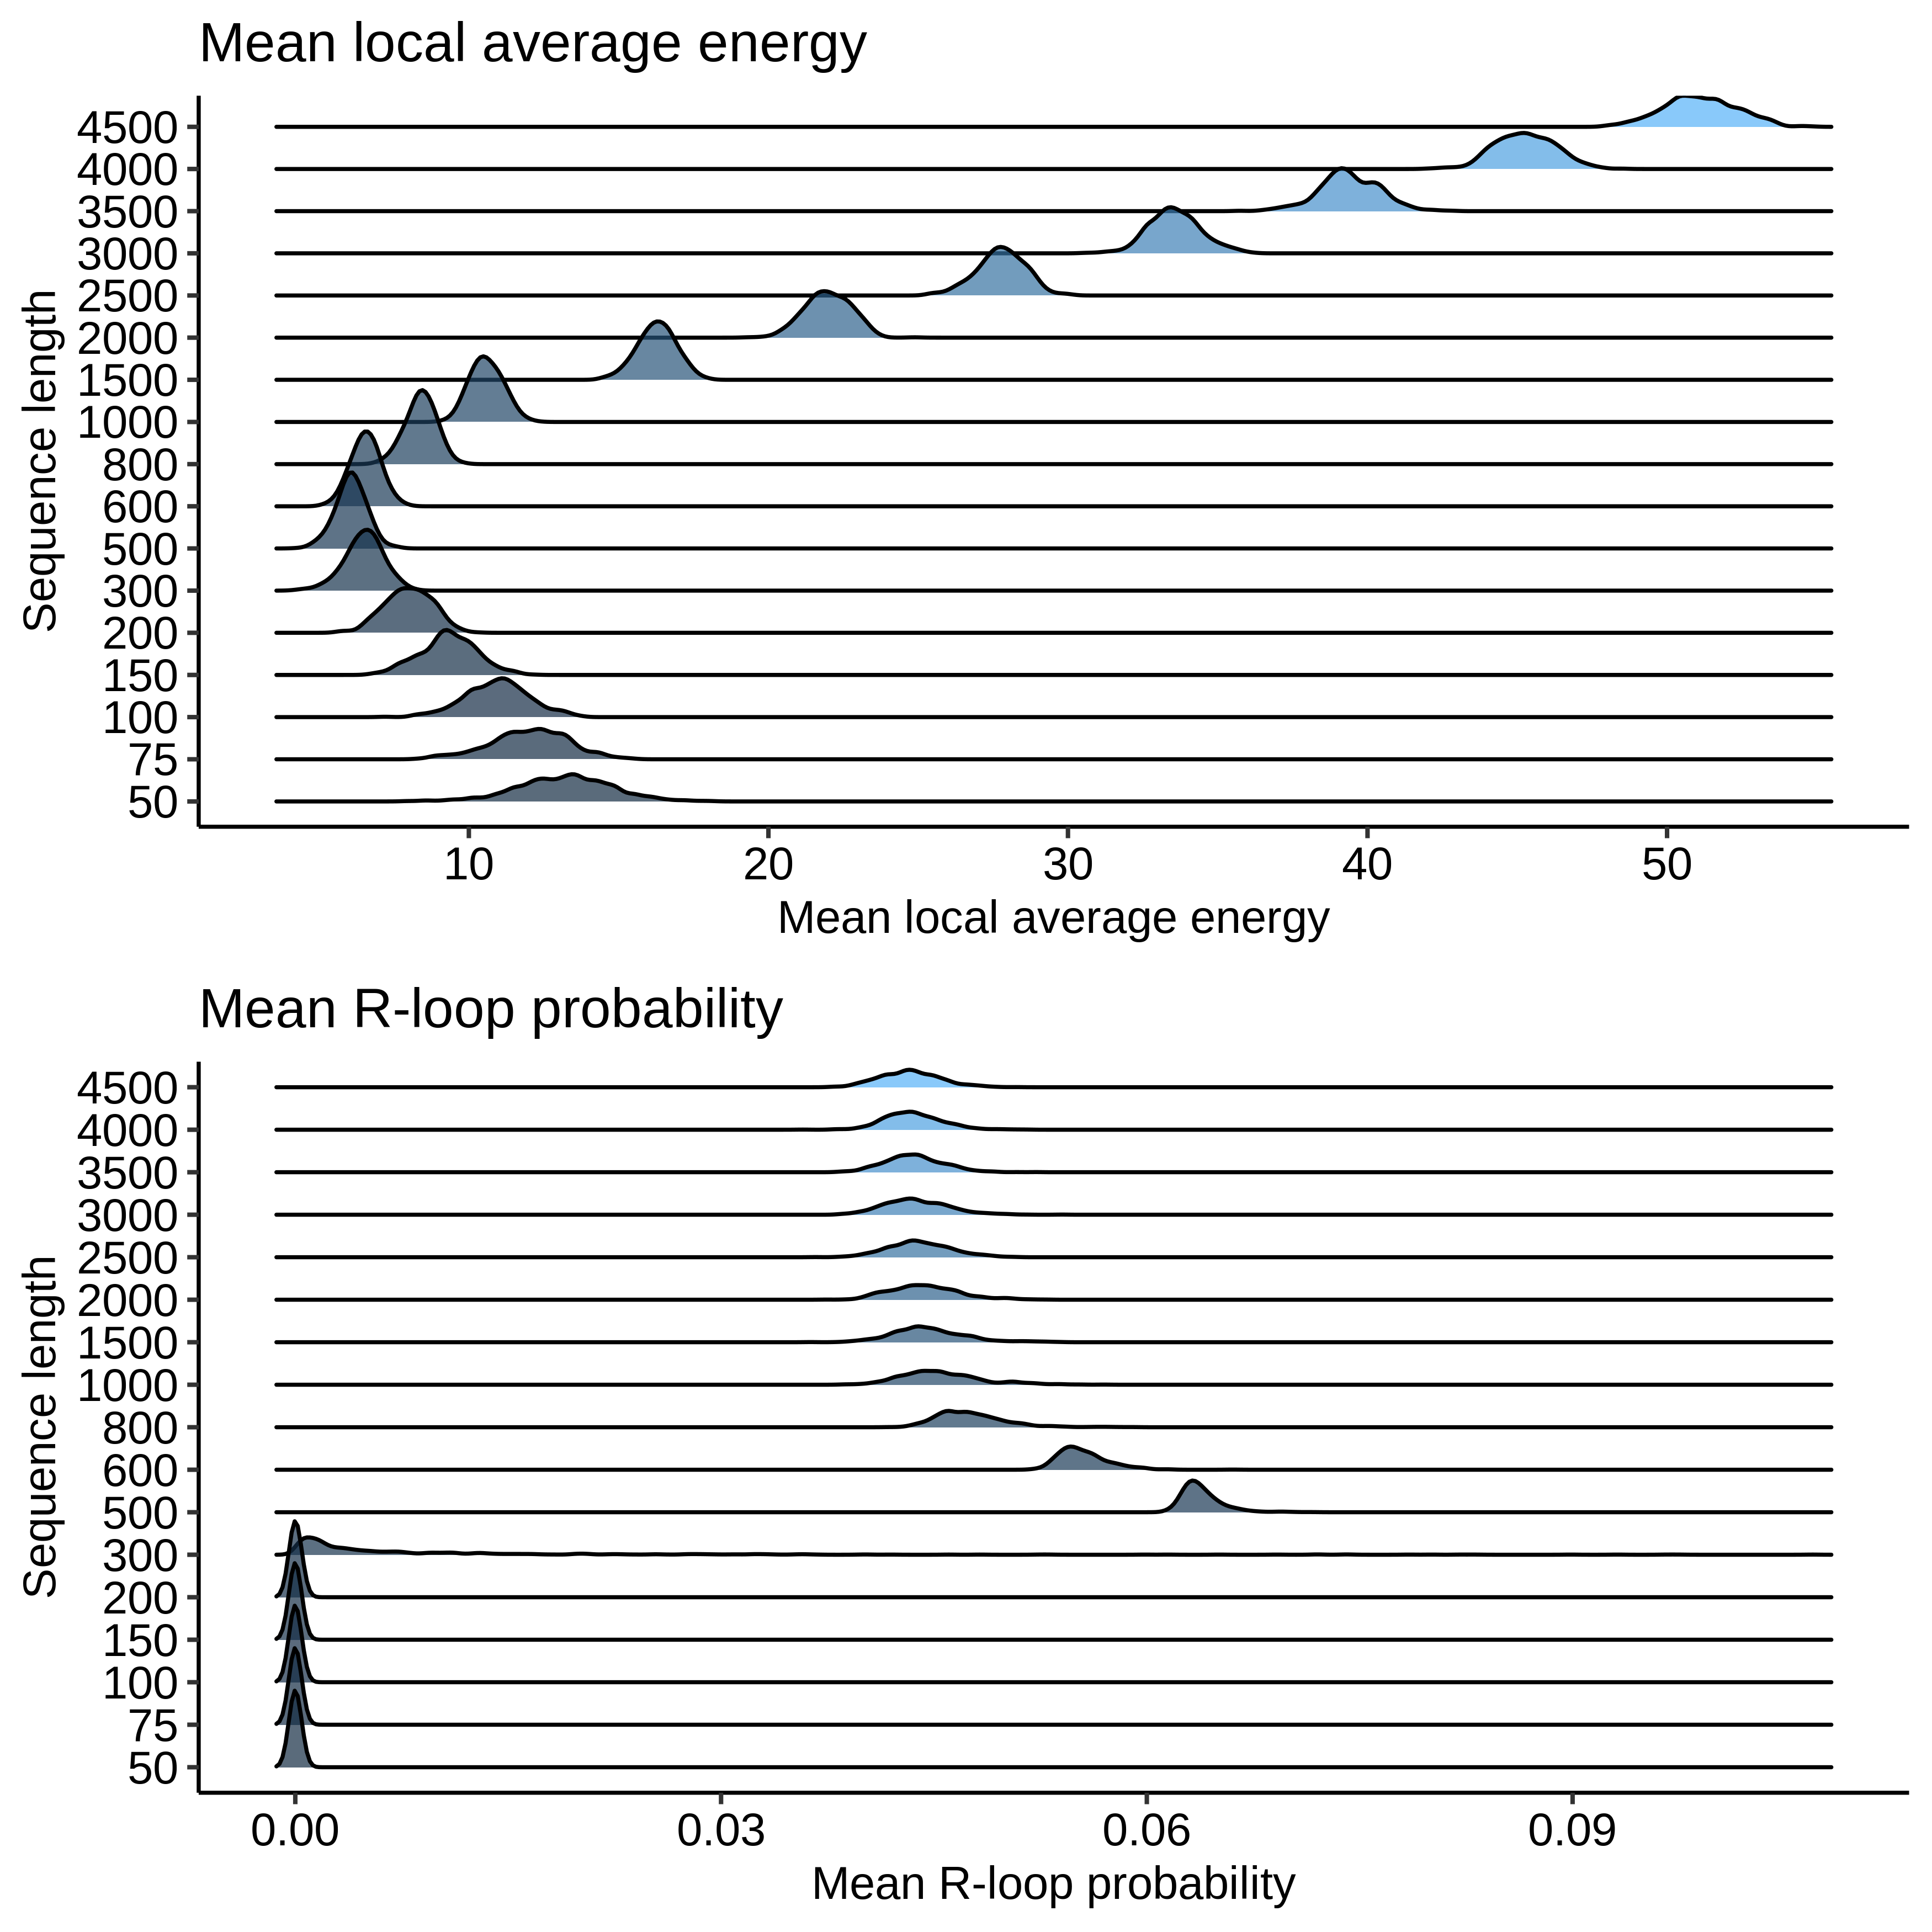
\includegraphics[width=15cm]{images/plots/rand_seq_LAE_dist.png}
	\centering
	\caption{Initial rlooper expectation plots based on completely random sequences.}
\end{figure}

The top figure shows the distribution of average R-loop energy for a given base pair, averaged over all R-loops that contain that base pair for random sequences of a given length.

Bottom plot

Thanks to conversations with Craig and Robert about this also decided using parameterized sequences would be more informative resulting in fig 1.


\subsection{Homology arm calculations}

Jupyter notebook that includes all code used to generate homology arms and insert
restriction sites is available  \href{https://github.com/EthanHolleman/plasmid-VR-design/blob/main/notes/homology_arms.ipynb}{at this link}. The genbank formatted files of both homology arms can be found in the same repository in the \href{https://github.com/EthanHolleman/plasmid-VR-design/tree/main/resources/files/genbank}{resources directory}.

\subsection{Variable regions in fasta format}
\label{sec:fasta-inserts}

\begin{verbatim}
>uI2oMODk-22mA4uMFkAWb8MNQEQ insert_init-1
TAGGGCGAATTGGAGCTCCACATCGGTACCCACGTTTGGCCACCATTAACTATATATGTA
TCCTTGCACACCCTTATCTAAATTGTCTTAGATTTTCAATCCTATAGTGTAGGTGTGGCA
GATGCAACTTTACAGGCGCGAGTTGGTACTACACGCAGACTAGTAATAGTGCAGTTTAGA
GAAGGGAAGAGGTAAATCGTCTAGTAAAACTAGGACTCTGTATAAGTTACCAACGGTGTT
ACCGCGAATTCGTCGCAGTGACCGAGGCGAGGAGG
>xxGE8Gg_FuXoRcMCzcbS8H6P8wk insert_init-2
TAGGGCGAATTGGAGCTCCACATCGGTACCCACGTTTGGCCACCACCTTCGCCGAATGGG
AAGCGGGGCAGGGGCCGGAGTCTAACCGAAGAGGGACAAGGGTCGACGCCGCTGGACGCG
GGGTAGGTTGGTTGTGGTCAGAGGGGCGGCGTGCGGGGGGCGGTGGCAACGTGGTATCGT
CGTCATGGACGTGACGCGCTGGGGGGCGATACACGGGGGGGGGGTGGCTTCAGAGTGCGG
TGGCCGAATTCGTCGCAGTGACCGAGGCGAGGAGG
>Qgaasm0lhlPX5b3t-z1qbJu3S9o insert_init-3
TAGGGCGAATTGGAGCTCCACATCGGTACCCACGTTTGGCCACCAATTATGGGGCTGGCT
ACGGAGGTGTAATTTCTAGGGAGGGGGAGCATTAGACGGTGGCAGGTTAGTGAGGGGGGG
GGACAGTCGAGCAGAGGCCGCGTATATGGGCGGGATGGTGGATGGACAAGGGAAGGTGCC
ACTCGAGGGTGGGTGTAAGGGGTGGTAGTTAGGAGGACTGGATTTGGCTGCGGTAGGGTG
GCACGGAATTCGTCGCAGTGACCGAGGCGAGGAGG
>HZfblNGgM64FV1hPYV8cTLZ5u0M insert_init-4
TAGGGCGAATTGGAGCTCCACATCGGTACCCACGTTTGGCCACCATGTGGTGCTGCGGCT
TGGGGAGGCGTCTTGTCGAGTGTCGATCGACAGGCGGTGGCCTGGGGGATCCGACTTCCG
GCTCCTTGGGGCCGCGCGAAGGGGGACATTCGGAGACACAGGGCCCGCTACCCCGCAGCG
AGCGGGGCGAAGCTGACCACGCAGCTCCCCCGTGCGACACGATGGCCTCCAGCGAGATCC
GGACCGAATTCGTCGCAGTGACCGAGGCGAGGAGG
>M3VLqJl5oQIRO7wZeEKKr_hUr40 insert_init-5
TAGGGCGAATTGGAGCTCCACATCGGTACCCACGTTTGGCCACCAACGCGGGATTGCCGG
ACATCGGAGAGCCCAACGAGCGGAATTTCCGTGACGAGGTCAGAGCTGATGGAACTCCCT
CAGTTACTCAGGTATGAACGTACTCAAAGGCCCTGTGTCGTGGGTGCACCGCTCCCTGGC
AGGGCTATTCCGCCGATACGCAGTCATCAGGGGACCGCGTGTTGCTACAACTGCCCCGTC
TCGTCGAATTCGTCGCAGTGACCGAGGCGAGGAGG
>Cyy1TuR8girckLFRFzzJQtffY78 insert_init-6
TAGGGCGAATTGGAGCTCCACATCGGTACCCACGTTTGGCCACCACACATTAGAGTACGT
AGAGGCACTGCATCCTGGGCGGTTTGAATTAGGTTAACTCGAGGGTAACTTGTACTTAAC
ATAGAGGAGAGGCATTCCACGCTTGGTCTCTAAAACTGTTTAGTATTGGGTAAACCCGAA
ATCTAATTTCAACGAGCTCTATAGGAAATAATTAATGGAAGATAGTGGTGTTATCGTTAC
ATTTGGAATTCGTCGCAGTGACCGAGGCGAGGAGG
>nnPuzS7AblFb1Bw2eAE_7h8SePY insert_init-7
TAGGGCGAATTGGAGCTCCACATCGGTACCCACGTTTGGCCACCAATTATGGGGCTGGCT
ACGGAGCTGTAATTTCTAGCCAGGGGGAGCATTAGACGGTGGCAGGTTACTGAGGGGGCG
CGACAGTCCAGCAGAGGCCGCGTATATGGGCGGGATGGTGGATGGACAAGGGAACGTGCC
ACTCGAGGCTGGGTGTAAGCGGTGGTACTTAGGAGGACTGGATTTGGCTGCGGTAGGCTG
GCACGGAATTCGTCGCAGTGACCGAGGCGAGGAGG
>48li-aMEdMWrqlvMwBVGdXkIoic insert_init-8
TAGGGCGAATTGGAGCTCCACATCGGTACCCACGTTTGGCCACCAAGCTAGAGTGTAGAT
GATCTAAGAATAGTATGGAGGGATTTAAGTGAGAGTTCGTAGAGGGAACTGCAGTGGCAG
GTGGGATGGAAATGTGAGCGTAGGTGTCTGCTTGGTAATAGGCTGGATCTGCAGGGTCGG
TGTCGGTGGGACTATGGGAGGGGTAATAGGCGCAAGCTGGGGTGATGCATAAGCGTTAAT
AGTTGGAATTCGTCGCAGTGACCGAGGCGAGGAGG
>k1DC5eUm6s6LHQ6IBWL3fh21sOU insert_init-9
TAGGGCGAATTGGAGCTCCACATCGGTACCCACGTTTGGCCACCAACGCGGGATTGCCGG
ACATCGGAGAGCCCAACGAGCGGAATTTCCGTGACGAGGTCAGAGCTGATGGAACTCCCT
CAGTTACTCAGGTATGAACGTACTCAAAGGCCCTGTGTCGTGGGTGCACCGGTCCCTGGC
AGGGCTATTCCGCCGATAGGCAGTCATGAGGGGACCGCGTGTTGCTACAACTGCCGGGTC
TCGTGGAATTCGTCGCAGTGACCGAGGCGAGGAGG
>PtfE-xW0Cu1CcZAF_GmNkRvARG8 insert_init-10
TAGGGCGAATTGGAGCTCCACATCGGTACCCACGTTTGGCCACCAACCTAGAGTCTACAT
CATCTAACAATACTATGGAGCGATTTAACTGAGAGTTCGTAGACCGAACTGCACTGGCAC
GTGGGATGCAAATGTGACCGTAGGTGTCTGCTTGCTAATAGGCTGGATCTGCAGGGTCGC
TGTCGCTCCCACTATCGGACGGGTAATAGGCGCAAGCTCGCCTCATCCATAACCCTTAAT
AGTTCGAATTCGTCGCAGTGACCGAGGCGAGGAGG
>ZfSsyr5JKJMmzfxVoihBQwhX_NE insert_init-11
TAGGGCGAATTGGAGCTCCACATCGGTACCCACGTTTGGCCACCATGTGGTGCTGCGGCT
TGGGGAGGGGTCTTGTGGAGTGTCGATCGAGAGGCGGTGGCCTGGGGGATCCGACTTCCG
GCTCCTTGGGGCCGCGCGAAGGGGGACATTCGGAGACACAGGGCCCGCTACCCCGGAGCG
AGCGGGGCGAAGGTGACCACGCAGCTCCGCCGTGCGACACGATGGCCTGCAGCGAGATCC
GGACCGAATTCGTCGCAGTGACCGAGGCGAGGAGG
>AB0ve2-vLjsIguhmvORXjxcgBfI insert_init-12
TAGGGCGAATTGGAGCTCCACATCGGTACCCACGTTTGGCCACCAATTATGGGGCTGGCT
ACGGATCTTTAATTTCTAGGCATGGGTATCATTAGACGTAGTCAGGTAACTGAGGGTGGG
CGACAGACGAGCAGAGGCCTCGAATAAGGGCTGGATGTAGGATGGACAAGTGAAGTTTCC
ACTCGAGGGTGGGAGTAAGGGGTGTTACTAATGATTACTGGAAATGGCTGCTGTATGCTG
GCACGGAATTCGTCGCAGTGACCGAGGCGAGGAGG
>0ajKeeoLFH_-_WR3FlsYUghJ_wo insert_init-13
TAGGGCGAATTGGAGCTCCACATCGGTACCCACGTTTGGCCACCAACGCGGGATTGCCGG
ACATCGGAGAGCGCAACGAGCGGAATTTCCGTGACGAGGTCAGAGCTGATGGAAGTCCGT
CAGTTAGTCAGGTATGAACGTACTCAAAGGCCCTGTGTGGTGGGTGCACCGGTCCCTGGC
AGGGCTATTCCGCCGATAGGCAGTCATGAGGGGACCGCGTGTTGCTACAAGTGCCGGGTC
TCGTGGAATTCGTCGCAGTGACCGAGGCGAGGAGG
>5vd9OwN61JjxUtv5yJRgi5W4rkQ insert_init-14
TAGGGCGAATTGGAGCTCCACATCGGTACCCACGTTTGGCCACCACTCATTACAGTACGT
TCACGCACTGCAGCCTCGGCGGTTGCAATTTGGTTAACTCGAGGGGAACTGCTACTTAAC
ATAGTGGAGACGCTTGCCACGCTGGCTCGCGATATCGGTGTAGTAGTGGCGAAACCCGAT
AGCTAATGTCAACGACCGCGTTACGTAATAAGGAATCGAAGATAGGGGTCTGATCGTTAC
ATTTGGAATTCGTCGCAGTGACCGAGGCGAGGAGG
>vOi3nAJBZKQbAAixEIhLho5HRG0 insert_init-15
TAGGGCGAATTGGAGCTCCACATCGGTACCCACGTTTGGCCACCATTAACTATATATGTA
TCCTTGCACACCCTTATCTAAATTGTCTTAGATTTTCAATCCTATAGTGTAGGTGTGGCA
GATGCAACTTTACAGGCGCGAGTTGCTACTACACCCAGACTAGTAATAGTGCAGTTTAGA
CAAGGGAAGAGGTAAATCGTCTACTAAAACTAGGACTCTGTATAAGTTACCAACGGTGTT
ACCGCGAATTCGTCGCAGTGACCGAGGCGAGGAGG
>F-umROlWXPNmCnU9huosc24irXk insert_init-16
TAGGGCGAATTGGAGCTCCACATCGGTACCCACGTTTGGCCACCAAAATGGAGAGGTTAG
TTGGAATTTGGCGTAGGTGAAGGCAAAAATAGAAATCGGTATAATGTTTCAAGGATGTTA
ACAAGGTGTGAAAGAGGTCGGTGACAGAAGTCTTTAAATAGTTATGTCTCAAATTACTCA
GTAGTTTGAGGAGGTATTGTAGGACGTTATTCCGATAGGGTTTATGTGCGTGATGGGGTG
GTGAGGAATTCGTCGCAGTGACCGAGGCGAGGAGG
>nfcEqNf7lCB4XRpZ2RAu70-sjy0 insert_init-17
TAGGGCGAATTGGAGCTCCACATCGGTACCCACGTTTGGCCACCACGTTCGCGGAATGGG
AAGCGGGGGAGGGGGGGGAGTCTAAGCGAAGAGGGACAAGGGTCGACGCCGGTGGACGCG
GGGTAGGTTGGTTGTGGTGAGAGGGGCGGGGTGCGGGGGGGGGTGGCAAGGTGGTATCGT
CGTGATGGAGGTGACGCGCTGGGGGGCGATACACGGGGGGGGGGTGGCTTCAGAGTGGGG
TGGCCGAATTCGTCGCAGTGACCGAGGCGAGGAGG
>xMIFrhuHyx0kfOAkHZv3Gt7avOM insert_init-18
TAGGGCGAATTGGAGCTCCACATCGGTACCCACGTTTGGCCACCAACTCGGGCGCGGAAG
GCAGCCACCGGCCCGAGGCCGTGTCCCCCGGGGCTTGGGCGTACAACTGGACTTCCCGGG
CGGAGGTCCTTCTCGACCACATAGACCGCGGCGGGAGGTGGGACGCCTTCCGTTTTAGCG
TCGTGCGCCGTAGGGCGAGGAGCTCCCGTTCAGACATCCAGGCTCGCAGCACATGCCCCC
GACCGGAATTCGTCGCAGTGACCGAGGCGAGGAGG
>_bPA1dDaKHyM7wwFymFjj8iaOHA insert_init-19
TAGGGCGAATTGGAGCTCCACATCGGTACCCACGTTTGGCCACCACACATTAGAGTACGT
AGAGGCAGTGCATCCTGGGCGGTTTGAATTAGGTTAACTCGAGGGTAAGTTGTACTTAAC
ATAGAGGAGAGGCATTCGAGGCTTGGTCTGTAAAACTGTTTAGTATTGGGTAAAGCGGAA
ATCTAATTTCAACGAGCTCTATAGGAAATAATTAATGGAAGATAGTGGTGTTATCGTTAG
ATTTGGAATTCGTCGCAGTGACCGAGGCGAGGAGG
>z-VWjJs4HOVPRiFTKkB2CMh0AeQ insert_init-20
TAGGGCGAATTGGAGCTCCACATCGGTACCCACGTTTGGCCACCAATTATGGGGCTGGCT
ACGGATCTTTAATTTCTAGCCATCGGTATCATTAGACGTAGTCAGCTAACTGAGGGTGCG
CGACAGACCAGCAGAGGCCTCGAATAAGGGCTGCATGTAGGATGGACAAGTGAACTTTCC
ACTCGAGGCTGCGAGTAAGCGGTGTTACTAATGATTACTGGAAATGGCTGCTGTATGCTG
GCACGGAATTCGTCGCAGTGACCGAGGCGAGGAGG
>a1rQbSGsl2x7SCwWDrGsQcxG2Jo insert_init-51
TAGGGCGAATTGGAGCTCCACATCGGTACCCACGTTTGGCCACCACACATTAGAGTACGT
AGAGGCACTGCATCCTGGGCGGTTTGAATTAGGTTAACTCGAGGGTAACTTGTACTTAAC
ATAGAGGAGAGGCATTCCAGGCTTGGTCTGTAAAACTGTTTAGTATTGGGTAAAGCGGAA
ATCTAATTTCAACGAGCTCTATAGGAAATAATTAATGGAAGATAGTGGTGTTATCGTTAC
ATTTGGAATTCGTCGCAGTGACCGAGGCGAGGAGG
>i5xBsEuOX_D3UAsMD5_D5RBKrRk insert_init-52
TAGGGCGAATTGGAGCTCCACATCGGTACCCACGTTTGGCCACCAAAAGGGAGAGGTTTG
GGGGAATTTGGCCTACCTGAAGGCTATAATAGAAATCGGTAGTATGTTGCAAGGTTCTTT
ACAACGTGTGAAAGTGGTCCGGGACACATCTCGTTAAATTCTGATGTCGCAAAGGACGCA
GTAGGTGCACGAGCTATTGTAGGACCTGATGCCGTTACGGTTGATCTCCGTGAGCGGCGG
GGGACGAATTCGTCGCAGTGACCGAGGCGAGGAGG
>Bl5NH1DmQHE_PhlW8RrNLnBKT24 insert_init-53
TAGGGCGAATTGGAGCTCCACATCGGTACCCACGTTTGGCCACCAACGCGGGATTGCCGG
ACATGGGAGAGCGCAACGAGCGGAATTTCCGTGACGAGGTCAGAGCTGATGGAAGTCCGT
CAGTTAGTGAGGTATGAAGGTACTCAAAGGGCCTGTGTGGTGGGTGCACCGGTCCGTGGC
AGGGCTATTCCGCCGATAGGCAGTCATGAGGGGAGCGCGTGTTGCTACAAGTGCCGGGTC
TCGTGGAATTCGTCGCAGTGACCGAGGCGAGGAGG
>BceLUjEU9O8GsQVx9xW1Kxn6SUI insert_init-54
TAGGGCGAATTGGAGCTCCACATCGGTACCCACGTTTGGCCACCAGCGCTGAACGGGGGA
GGGTCGGGGCGGGCGGCGTGAGAGCTCAGGCTCCGGGGTGTACGGGAGGTGCAGGGGGGC
GCATCCATGGGTAGGCGGGAGGCAAAGTATCGAAGGGCCCACAGATGGGTCGTTGTCCGT
GGAGTTCGCTGACCTCTGCACCCGCGGCTGAGCCGGGGGTCCCCGCACGGAGTTGGATGG
GTCCAGAATTCGTCGCAGTGACCGAGGCGAGGAGG
>kSnZfaYyMmtaXNeKUrJYDrVc6is insert_init-55
TAGGGCGAATTGGAGCTCCACATCGGTACCCACGTTTGGCCACCATTAACTATATATGTA
TGGTTGCAGACCGTTATGTAAATTGTCTTAGATTTTCAATCGTATAGTGTAGGTGTGGCA
GATGGAACTTTAGAGGCGCGAGTTGGTACTACAGGGAGACTAGTAATAGTGGAGTTTAGA
GAAGGGAAGAGGTAAATGGTCTAGTAAAACTAGGACTGTGTATAAGTTACCAAGGGTGTT
ACGGGGAATTCGTCGCAGTGACCGAGGCGAGGAGG
>izktT5yxYm4tK4Ise9OtCjMWvoA insert_init-56
TAGGGCGAATTGGAGCTCCACATCGGTACCCACGTTTGGCCACCAAGCTAGAGTGTAGAT
GATCTAAGAATAGTATGGAGGGATTTAACTGAGAGTTCGTAGAGGGAACTGCAGTGGCAC
GTGGGATGGAAATGTGAGCGTAGGTGTCTGCTTGGTAATAGGCTGGATCTGCAGGGTCGC
TGTCGGTGGGACTATCGGAGGGGTAATAGGCGCAAGCTGGGGTGATGCATAAGCGTTAAT
AGTTCGAATTCGTCGCAGTGACCGAGGCGAGGAGG
>D_X_8FNcqgcekMkN6HwwXxxeSWo insert_init-57
TAGGGCGAATTGGAGCTCCACATCGGTACCCACGTTTGGCCACCAAGTGGATCATGGTGT
TGGGTATTGTTCTTGAGGAGTGAGGATCGAGAGGGGGTGGGCTGGGGGAAGCGACAACCG
GCTGGAAGTGTCGGGGGGAAGGGGGAGATTCTGAGAGAGAGTGGGCTCTACCGCGGAGCG
AGGGTGGCTAAGGTGACCACTGATGTGCGCCGTGGTACACTATGTCGTGGATGGAGATCC
GGACGGAATTCGTCGCAGTGACCGAGGCGAGGAGG
>LrNW4QmsWQQFWxdEJX_k9mBQBCo insert_init-58
TAGGGCGAATTGGAGCTCCACATCGGTACCCACGTTTGGCCACCAATGTGGGGGCGGGCT
TCGGAGCGGTTAGGGCGAGCCAGGGGGAGCAGGTGACGGTGGCAGGGTTCGGAGGGGGCG
CGTCAGTCCAGCAGTGGCCGCGTTGATGGGCGGGATGGTGGATGGACATGGGAAGGGGCC
TCTCGAGGCGGGGTGTAAGCGGGGGGACGTAGGAGGACTGGATTGGGCGGCGGTAGGCTG
GCACGGAATTCGTCGCAGTGACCGAGGCGAGGAGG
\end{verbatim}

\subsection{Complete inserts in fasta format}


\subsection{RNA secondary structure expectation plots}




\pagebreak

\bibliography{refs/refs.bib}

\end{document}
